\documentclass{dissertation}
%\documentclass[print]{dissertation}
%\documentclass[print,draft]{dissertation}

\hyphenation{TestRoots WatchDog proj-ect proj-ects Ec-lipse two-fold clie-nts Mo-cki-to wide-spread}
\newcommand{\sparkline}[1]{$\vcenter{\hbox{\includegraphics[scale=0.04]{#1}}}$}

\makeglossaries

\newcommand*{\origrightarrow}{}
\let\oldarrow\textrightarrow
\renewcommand*{\textrightarrow}{\fontfamily{cmr}\selectfont\origrightarrow}
\loadglsentries[main]{glossary}

\usepackage{xspace}

% abbreviations for programs
\newcommand\maven{\textsc{Maven}\xspace}
\newcommand\gradle{\textsc{Gradle}\xspace}
\newcommand\ant{\textsc{Ant}\xspace}
\newcommand\junit{\textsc{JUnit}\xspace}
\newcommand\testng{\textsc{TestNG}\xspace}
\newcommand\rspec{\textsc{RSpec}\xspace}

\newcommand\git{\textsc{git}\xspace}

\newcommand\travis{\textsc{Travis CI}\xspace}
\newcommand\docker{\textsc{Docker}\xspace}
\newcommand\github{\textsc{GitHub}\xspace}
\newcommand\ghtorrent{\textsc{GHTorrent}\xspace}
\newcommand\mongo{\textsc{MongoDB}\xspace}

\newcommand\testroots{\textsc{TestRoots}\xspace}
\newcommand\watchdog{\textsc{Watch\-Dog}\xspace}
\newcommand\wdog{\textsc{WD}\xspace}
\newcommand\watchdogt{\textsc{Watch\-Dog 2.0}\xspace}

\newcommand\feedbag{\textsc{Feed\-BaG++}\xspace}
\newcommand\fbag{\textsc{FB}\xspace}

\newcommand\gnuparallel{\textsc{GNU Parallel}\xspace}

\newcommand\buildanalyzer{\textsc{Buildlog Analyzer}\xspace}
\newcommand\travispoker{\textsc{Travis Poker}\xspace}
\newcommand\travisharvester{\textsc{Travis Harvester}\xspace}
\newcommand\ghanalyzer{\textsc{GitHub Analyzer}\xspace}


\newcommand\rubocop{\textsc{RuboCop}\xspace}
\newcommand\findbugs{\textsc{FindBugs}\xspace}
\newcommand\pmd{\textsc{PMD}\xspace}
\newcommand\jscs{\textsc{JSCS}\xspace}
\newcommand\jshint{\textsc{JSHint}\xspace}
\newcommand\eslint{\textsc{ESLint}\xspace}
\newcommand\jsl{\textsc{JSL}\xspace}
\newcommand\pylint{\textsc{Pylint}\xspace}
\newcommand\checkstyle{\textsc{Checkstyle}\xspace}
\newcommand\coverity{\textsc{Coverity}\xspace}

\newcommand\eclipse{\textsc{Eclipse}\xspace}
\newcommand\intellij{\textsc{IntelliJ}\xspace}
\newcommand\visualstudio{\textsc{Visual Studio}\xspace}
\newcommand\netbeans{\textsc{Netbeans}\xspace}

\newcommand\travistorrent{\textsc{TravisTorrent}\xspace}

\newcommand\uav{\textsc{UAV}\xspace}


\begin{document}

%% Specify the title and author of the thesis. This information will be used on
%% the title page (in title/title.tex) and in the metadata of the final PDF.
%\title{Optimizing the Performance of Distributed Systems With Accountability}
\title{Practical Accountability and Fraud Detection in Distributed Systems}
\author{Marinus Abraham}{de Vos}

%% Use Roman numerals for the page numbers of the title pages and table of
%% contents.
\frontmatter

\begin{titlepage}

\begin{center}

%% Extra whitespace at the top.
\vspace*{2\bigskipamount}

%% Print the title.
\begin{spacing}{1.6}
{\makeatletter
\titlestyle\bfseries\LARGE\@title
\makeatother}
\end{spacing}

%% Print the optional subtitle.
{\makeatletter
\ifx\@subtitle\undefined\else
    \bigskip
    \titlefont\titleshape\Large\@subtitle
\fi
\makeatother}

\end{center}

\cleardoublepage
\thispagestyle{empty}

\begin{center}

%% The following lines repeat the previous page exactly.

\vspace*{2\bigskipamount}

%% Print the title.
\begin{spacing}{1.6}
{\makeatletter
\titlestyle\bfseries\LARGE\@title
\makeatother}
\end{spacing}

%% Print the optional subtitle.
{\makeatletter
\ifx\@subtitle\undefined\else
    \bigskip
    \titlefont\titleshape\Large\@subtitle
\fi
\makeatother}

%% Uncomment the following lines to insert a vertically centered picture into
%% the title page.
%\vfill
%\includegraphics{title}
\vfill

%% Apart from the names and dates, the following text is dictated by the
%% promotieregelement.

{\Large\titlefont\bfseries Proefschrift}

\bigskip
\bigskip

ter verkrijging van de graad van doctor

aan de Technische Universiteit Delft,

op gezag van de Rector Magnificus prof.~dr.~ir.~T.H.J.J.~van~der~Hagen,

voorzitter van het College voor Promoties,

in het openbaar te verdedigen

op woensdag 16 juni 2021 om 17:30 uur

\bigskip
\bigskip

door

\bigskip
\bigskip

%% Print the full name of the author.
\makeatletter
{\Large\titlefont\bfseries\@firstname\ \titleshape{\MakeUppercase{\@lastname}}}
\makeatother

\bigskip
\bigskip

Master of Science in Computer Science, \\
Technische Universiteit Delft, Nederland,

geboren te Sint-Maartensdijk, Nederland.

%% Extra whitespace at the bottom.
\vspace*{2\bigskipamount}

\end{center}

\clearpage
\thispagestyle{empty}

%% The following line is dictated by the promotieregelement.
\noindent Dit proefschrift is goedgekeurd door de

%% List the promotors (supervisors).
\medskip\noindent
\begin{tabular}{l}
    promotor: Prof.dr.ir.\ D.H.J.\ Epema \\
    promotor: Dr.ir.\ J.A.\ Pouwelse
\end{tabular}

\bigskip
\noindent Samenstelling promotiecommissie:

%% List the committee members, starting with the Rector Magnificus and the
%% promotor(s) and ending with the reserve members.
\medskip\noindent
\begin{tabular}{p{4.5cm}l}
    Rector Magnificus, & voorzitter \\
    Prof.dr.ir.\ D.H.J. Epema, & Technische Universiteit Delft, promotor\\
    Dr.ir.\ J.A. Pouwelse, & Technische Universiteit Delft, promotor\\

    \medskip
    \mbox{\emph{Onafhankelijke leden:}} & \\
    Prof.dr.\ A. van Deursen, & Technische Universiteit Delft \\
    Prof.dr.\ A.M. Kermarrec, & École polytechnique fédérale de Lausanne, Switzerland \\
    Prof.dr.\ F.\ Taïani, & Université de Rennes 1, France \\
    Dr.\ A.\ Gervais, & Imperial College London, United Kingdom \\
    Dr.\ D.G.J. Bongaerts, & Erasmus University Rotterdam \\
    
    Prof.dr.\ K.G. Langendoen & Technische Universiteit Delft, reservelid \\ \\

\end{tabular}

%% Include the following disclaimer for committee members who have contributed
%% to this dissertation. Its formulation is again dictated by the
%% promotieregelement.
%\medskip
%\noindent  %Prof.\ Dr.\ D.\ Spinellis has contributed to the creation of this thesis.

\medskip
\medskip
% TODO Include http://www.win.tue.nl/ipa/?page_id=309
%\noindent The work in the thesis has been carried out under the auspices of the research school ASCI (Advanced School for Computing and Imaging).

\medskip
%% Here you can include the logos of any institute that contributed financially
%% to this dissertation.
\vfill
\begin{center}
    
\includegraphics[height=0.5in]{title/logos/tudelft}
    \hspace{2em}
    %
\includegraphics[height=0.5in]{title/logos/casimir} \\
%    
\includegraphics[height=0.5in]{title/logos/nwo}
    \\ \vspace{0.5cm}
%    
\includegraphics[height=0.5in]{title/logos/ipa}
\end{center}
\vfill

\noindent
\begin{tabular}{@{}p{0.2\textwidth}@{}p{0.8\textwidth}}
  \textit{Keywords:} & decentralization, disintermediation, electronic markets, e-commerce, blockchain, decentralized exchanges, matchmaking, settlement, fraud, information management, identity management, decentralized finance, trading, money \\[\medskipamount]
      \textit{Printed by:} & \todo{TBD} \\[\medskipamount]
      \textit{Cover:} & \todo{TBD}  \\[\medskipamount]
      \textit{Style:} & TU Delft House Style, with modifications by Moritz Beller \\& \url{https://github.com/Inventitech/phd-thesis-template} \\[\medskipamount]
\end{tabular}

\medskip
\medskip
\noindent The author set this thesis in \LaTeX\xspace using the Libertinus and Inconsolata fonts.

\vspace{\bigskipamount}

% Copyrighting this is stupid, questionable, and probably illegal, because large parts of the
% thesis have already been published with the copyright resigning with the publisher.
%\noindent Copyright \textcopyright\ 2015 by A.~Einstein

%% Uncomment the following lines if this dissertation is part of the Casimir PhD
%% Series, or a similar research school.
%\medskip
%\noindent Casimir PhD Series, Delft-Leiden 2015-01

%\medskip
\noindent ISBN \todo{TBD}

\medskip
\noindent An electronic version of this dissertation is available at \\
\url{http://repository.tudelft.nl/}.

\end{titlepage}



%% The (optional) dedication can be used to thank someone or display a
%% significant quotation.
%\dedication{\epigraph{I [...] like to give the maximum in everything I do. The maximum I have. The
%    maximum I can give. I am not perfect. But if I do something, I do it [as best I can].
%    %And many people are not made like this. There are only few. But I like these few.
%  }{Reinhold Messner}}

\tableofcontents

\chapter*{Summary}
\addcontentsline{toc}{chapter}{Summary}
\setheader{Summary}

\dropcap{M}arketplaces facilitate the exchange of services, goods and information between individuals and businesses.
They play an essential role in our economy.
The standard approach to devise digital marketplaces is by deploying centralized infrastructure, entirely operated and managed by a market operator.
In such centralized marketplaces, trusted intermediaries often provide various services to traders, such as managing market information, processing payments, and providing arbitration services when a dispute arises.

Advancements in information technology have challenged the need for both authoritative market operators and trusted intermediaries.
In particular, blockchain technology is increasingly being applied to deploy digital marketplaces.
Blockchain-based marketplaces facilitate trade directly between peers while reducing the dependency on both authoritative parties and trusted intermediaries.
The role of blockchain in such marketplaces is to replace social trust with cryptographic primitives.
This enables the \emph{decentralization} and \emph{disintermediation} of different components in digital marketplaces.
In the context of this thesis, decentralization refers to the concept of delegating decision making and activities away from a central authority.
Disintermediation reduces or removes the involvement of trusted intermediaries when trading on a digital marketplace.

This thesis introduces innovative approaches to decentralize and disintermediate all aspects of blockchain-based marketplaces.
We first identify the five aspects of blockchain-based marketplaces: information management, matchmaking, settlement, fraud management, and identity management.
We then design, implement, evaluate, and deploy five decentralized mechanisms.
Each introduced mechanism focusses on one or two aspects of blockchain-based marketplaces.
For each mechanism, we consider feasibility and real-world deployment as crucial requirements for successful adoption.

In Chapter 1 we identify and describe the five aspects of blockchain-based marketplaces.
We outline existing approaches that disintermediate and decentralize these aspects.
We then formulate our research questions, describe our research and engineering methodology, and summarize the key contributions of this thesis.

In Chapter 2 we introduce a universal accounting mechanism, named \emph{\TrustChain{}}, to securely store information in decentralized applications.
With \TrustChain{}, each peer maintains a personal ledger containing tamper-evident records.
A record describes an agreement between peers and links to other records.
Fraud, the illegitimate modification of a record in one's personal ledger, is detected by continuously exchanging records and by verifying the consistency of incoming records against known ones.
We experimentally show that \TrustChain{} is highly scalable and that fraud can be detected quickly.
To highlight the applicability of our work, we perform a two-year deployment trial of \TrustChain{} to address free-riding behaviour in \Tribler{}, our decentralized file-sharing application.
We leverage the accounting capabilities of \TrustChain{} for other mechanisms introduce in this thesis.

In Chapter 3 we introduce \emph{MATCH}, a decentralized middleware for fair matchmaking in peer-to-peer markets.
MATCH addresses manipulation concerns associated with marketplaces under central control, namely the ability by the market operator to prioritize, hide, or delay specific orders.
By decoupling the dissemination of potential matches from the negotiation of trade agreements, MATCH empowers end users to make their own educated decisions and to engage in direct negotiations with trade partners.
We evaluate MATCH with real-world ride-hailing and asset trading workloads.
Our experiments demonstrate that MATCH is highly resilient against malicious matchmakers that deviate from a specific matching policy.

In Chapter 4 we introduce a universal and decentralized settlement mechanism named \emph{XChange}.
This mechanism enables the exchange of assets between permissioned blockchains without the requirement for a trusted intermediary, collateral deposits, or modifications to deployed blockchain applications.
XChange records the progression of each trade within records on a distributed log.
To address counterparty risk, XChange bounds the economic gains of adversaries that have committed fraud during a trade by preventing them from engaging in other trades.
By inspecting the trade records in the distributed log, every participant can detect if a trader is refraining from fulfilling its obligations during an ongoing trade.
Our evaluation shows that XChange is highly scalable and has low overhead, while reducing economic losses by more than 99\%.

In Chapter 5 we introduce \emph{Internet-of-Money}, a settlement mechanism for real-time and international money transfers between different banks.
The key idea is to break up a slow inter-bank payment into multiple fast intra-bank payments.
Each money transfer uses one or more volunteer-based services, named money routers, to complete an intra-bank payment.
This approach reduces the duration of inter-bank payments from days to mere seconds.
To identity fraud, i.e., not forwarding incoming money as a router to the beneficiary, all transfer operations by users and money routers are recorded in a distributed log.
To further reduce risks, we break up a single money transfer into multiple smaller ones and leverage multiple money routers in parallel.
Our experiments show that these approaches significantly reduce fraud gains by adversarial parties.

In Chapter 6 we introduce \emph{\Dappcoder{}}, a decentralized crowdsourcing marketplace for the development of decentralized applications.
\Dappcoder{} addresses fragmentation and lock-in effects associated with centralized marketplaces for crowdsourcing.
A key part of \Dappcoder{} is DevID, a blockchain-based identity solution for software developers.
DevID unifies developer information within records on a distributed log.
Developers can import data assets from third parties into a unified DevID portfolio, add projects and skills, and receive endorsements.
Clients can leverage the \Dappcoder{} marketplace to create and manage projects, and to directly remunerate developers with cryptocurrencies while avoiding the need for trusted intermediaries.
Our user trial demonstrates that both \Dappcoder{} and DevID are efficient at storing and managing data.

Finally, in Chapter 7, we formulate the main conclusions of this thesis and present suggestions for further research directions.

\chapter*{Samenvatting}
\addcontentsline{toc}{chapter}{Samenvatting}
\setheader{Samenvatting}

{\selectlanguage{dutch}

\dropcap{M}arkten faciliteren het verhandelen van diensten, goederen en informatie tussen individuen en bedrijven.
Ze spelen een essentiële rol in onze economie.
De standaard werkwijze om elektronische markten in te richten is door het gebruik van gecentraliseerde infrastructuur die volledig geopereerd en beheerd wordt door een marktexploitant.
In dergelijke markten zijn er vaak vertrouwde tussenpartijen die verschillende diensten aanbieden aan gebruikers, zoals het beheren van marktinformatie, het verwerken van betalingen en het uitvoeren van arbitrage bij een geschil.

Innovaties in de informatietechnologie hebben de behoefte aan vertrouwde tussenpartijen in twijfel getrokken.
Met name blockchaintechnologie wordt steeds vaker toegepast om elektronische markten te creëren.
Blockchain-gebaseerde marktplaatsen faciliteren directe handel tussen gebruikers en verminderen de afhankelijkheid van zowel gezaghebbende partijen als vertrouwde tussenpartijen.
De rol van blockchain op dergelijke marktplaatsen is om sociaal vertrouwen te vervangen door cryptografische algoritmes.
Dit maakt de \emph{decentralisatie} en \emph{disintermediatie} van verschillende componenten in elektronische marktplaatsen mogelijk.
In de context van dit werk betekent decentralisatie het verminderen van besluitvorming en activiteiten die worden uitgevoerd door een centrale autoriteit.
Disintermediatie vermindert of verwijdert de betrokkenheid van vertrouwde tussenpartijen bij het handelen op een elektronische markt.

Dit proefschrift introduceert innovatieve mechanismes om alle aspecten van blockchain-gebaseerde markten te decentraliseren en te disintermediëren.
We identificeren eerst de vijf aspecten van blockchain-gebaseerde markten: informatiebeheer, matchmaking, de afwikkeling van handel, het afhandelen van fraude en het beheren van identiteit.
Vervolgens ontwerpen, implementeren en evalueren we vijf gedecentraliseerde mechanismen.
Elk geïntroduceerd mechanisme richt zich op één of twee aspecten van blockchain-gebaseerde markten.
Voor elk mechanisme beschouwen we een praktisch nut en een bijhorende implementatie als cruciale vereisten voor een succesvolle acceptatie.

In hoofdstuk 1 identificeren en beschrijven we de vijf aspecten van marktplaatsen die op blockchain gebasseerd zijn.
We beschrijven bestaande oplossingen die deze aspecten disintermediëren en decentraliseren.
Vervolgens formuleren we onze onderzoeksvragen, beschrijven we onze onderzoeks- en ontwikkelmethodologie en vatten we de belangrijkste bijdragen van dit proefschrift samen.

In hoofdstuk 2 introduceren we een universeel mechanisme genaamd \emph{\TrustChain{}}, voor het bijhouden van informatie in decentrale netwerken.
Met \TrustChain{} houdt elke gebruiker een persoonlijk grootboek met records bij.
Een record bevat een contractuele overeenkomst tussen gebruikers en bevat ook verwijzingen naar andere records in het grootboek.
Fraude, het onwettig wijzigen van een record in iemands persoonlijke grootboek, wordt gedetecteerd door continu records uit te wisselen en door de consistentie van inkomende records met reeds opgeslagen records te verifiëren.
We laten met experimenten zien dat \TrustChain{} zeer schaalbaar is en dat fraude snel kan worden gedetecteerd.
Om de toepasbaarheid van ons werk te evalueren voeren we een tweejarige pilot uit van \TrustChain{} om meelifters (free-riders) aan te pakken in Tribler, onze gedecentraliseerde applicatie voor het delen van bestanden.
We maken gebruik van de mogelijkheden van \TrustChain{} voor andere mechanismen die in dit proefschrift worden geïntroduceerd.

In hoofdstuk 3 introduceren we \emph{MATCH}, een gedecentraliseerde middleware voor eerlijke matchmaking in peer-to-peer markten.
MATCH pakt manipulatieproblemen aan die verband houden met marktplaatsen onder centrale controle, namelijk de mogelijkheid om specifieke orders door de marktexploitant te prioriseren, te verbergen of te vertragen.
Door de verspreiding van potentiële matches los te koppelen van de onderhandelingen over handelsovereenkomsten, stelt MATCH eindgebruikers in staat hun eigen weloverwogen beslissingen te nemen en directe onderhandelingen met handelspartners aan te gaan.
We evalueren MATCH met zowel een ride-hailing als een token trading dataset.
Uit onze experimenten blijkt dat MATCH zeer resistent is tegen kwaadwillende matchmakers die afwijken van een specifiek matching beleid.

In hoofdstuk 4 introduceren we een universeel en gedecentraliseerd mechanisme voor settlement, genaamd \emph{XChange}.
Ons mechanisme maakt de uitwisseling van tokens tussen blockchains met explicitiet geautoriseerde toegang mogelijk zonder een vertrouwde tussenpersoon, onderpanddeposito's of wijzigingen aan geïmplementeerde applicaties op de blockchain.
XChange registreert de voortgang van elke transactie in een gedistribueerd grootboek.
Om het tegenpartijrisico te verkleinen, beperkt XChange de economische winsten van kwaadwillige gebruikers die fraude hebben gepleegd door te voorkomen dat ze andere transacties aangaan.
Door het gedistribueerde grootboek te inspecteren, kan elke gebruiker detecteren of een handelaar heeft afgezien van het nakomen van zijn of haar verplichtingen tijdens een lopende transactie.
Onze resultaten tonen aan dat XChange zeer schaalbaar is en de economische verliezen van gedupeerde gebruikers met meer dan 99\% reduceert.

In hoofdstuk 5 introduceren we \emph{Internet-of-Money}, een mechanisme voor realtime en internationale geldovermakingen tussen verschillende banken.
Het idee is om een ​​langzame interbancaire betaling op te splitsen in meerdere snelle intrabancaire betalingen.
Elke geldoverdracht maakt gebruik van één of meer op vrijwilligers gebaseerde diensten, geldrouters, om een ​​betaling binnen de bank te voltooien.
Deze benadering reduceert de duur van interbancaire betalingen van dagen tot louter seconden.
Om fraude, d.w.z. het niet doorsturen van inkomend geld als router naar de volgende gebruiker, worden alle betalingen tussen gebruikers en geldrouters geregistreerd in een gedistribueerd grootboek.
Om de risico's verder te verkleinen, splitsen we een enkele betaling op in meerdere kleinere betalingen en gebruiken we voor een transactie meerdere geldrouters tegelijkertijd.
Onze experimenten tonen aan dat deze aanpak de winsten voor kwaadwillige gebruikers aanzienlijk vermindert.

In hoofdstuk 6 introduceren we \emph{\Dappcoder{}}, een marktplaats voor het crowdsourcen van de ontwikkeling van gedecentraliseerde applicaties.
\Dappcoder{} pakt fragmentatie- en lock-in-effecten aan die verband houden met gecentraliseerde marktplaatsen voor crowdsourcing.
Een belangrijk onderdeel van \Dappcoder{} is DevID, een op blockchain gebaseerde identiteitsoplossing voor softwareontwikkelaars.
DevID verenigt ontwikkelaarsinformatie en slaat deze informatie op in records in een gedistribueerd grootboek.
Ontwikkelaars kunnen gegevens van derde partijen importeren in een DevID portfolio, projecten en vaardigheden toevoegen en aanbevelingen voor vaardigheden ontvangen.
Gebruikers kunnen \Dappcoder{} benutten om projecten te maken en te beheren, en om ontwikkelaars te belonen voor hun werkzaamheden zonder tussenpartijen.
Onze pilot toont aan dat zowel \Dappcoder{} als DevID efficiënt zijn in het opslaan en beheren van gegevens.

Ten slotte formuleren we in hoofdstuk 7 de belangrijkste conclusies van dit proefschrift en doen we suggesties voor toekomstige onderzoeksrichtingen.
}




\chapter*{Acknowledgments}
\addcontentsline{toc}{chapter}{Acknowledgments}
\setheader{Acknowledgments}

While it is often said that a PhD is a lonely and though process, I very much enjoyed most aspects of it.
However, I would not have completed this journey were it not for the continuous support by many great people!

I would like to thank Johan Pouwelse, my promotor and daily supervisor.
Under your supervision, there has not been a single day where I was bored with my research or ran out of ideas, even after yet another paper rejection.
Our random and unorganized discussions, whether or not with other lab members, have been a great source of inspiration.
Your leadership and advice has helped me tremendously to become an independent researcher and to get my ideas published in the scientific community, which was definitely not always easy.
I highly value your relentless focus on practicality and usability (\enquote{no passing grade without running code}).
I enjoyed the freedom that you give every individual member of the lab to explore new ideas, and I am grateful for the many opportunities you gave me to (co-)supervise BSc and MSc students.

I would like to express my gratitude to my promotor Dick Epema, who was always willing to bring my research work to the next level by identifying both fundamental flaws and minor presentation issues.
Your knowledge, together with detailed and critical feedback has helped me to improve my writing style, my research papers and this thesis.

I thank all my collegues for making the office life very enjoyable.
Quinten, Egbert, and Sandip: I fondly remember the work we did on Tribler and the conversations we had since 2016 in our old office, whether or not around the coffee machine.
Bulat, thank you for the many chats we had about our research, science, and other topics.
Can, Georgy and Mitchell, thank you for your help as co-author on various papers.
I also thank Georgy for providing many insights from a socio-technological perspective on the work we produce as lab.
Ayman, thank you for inviting me to work together on an energy trading platform, I've learned many new things about your field!
I would also like to thank Elric, Vadim, Alexander and Andrew for our collaboration on Tribler.
Tamara, Kim and Sophie: thank you for taking care of our administrative burdens!
I also would like to thank the graduate school for the opportunity to physically defend my thesis during the ongoing pandemic.

Besides the people directly involved in my research, I would like to extend my gratitude to a large group of people with whom I spent many Wednesday evening playing games, eating pizza and/or drinking in the /pub and the Doerak.
These evenings were very helpful in unwinding from the hectic academic life.
Otto, thank you for the many conversions and coffee/beer talks that we had!
I would also like to thank Stefan, Jesse, Hans, Ernst, Maria, Thomas, Gijs, Tim, Chris, Jetse, Alexander, Taraneh, and others who occasionally joined for the Wednesday evening (there are just too many to list here!).

I am grateful for the many memories I made with friends.
Laurens, thank you for the many projects we worked on, the games we played, the tv shows we watched (most of which seem to be cancelled for some reason), and in general for great memories since I started my BSc in Delft!
Laurens, Anton and Martijn: thank you for the amazing trips during summer and winter holidays that we made across the world, whether or not accompanied by others.
I will never forget that feeling after we (finally) reached the summit of Mount Fuji!\emojifuji{}

Last, but definitely not least, I would like to thank my parents for their continuous support.
I would also like to thank Walter for teaching me many new skills during the construction of our \enquote{emergency} apartment.

\begin{flushright}
{\makeatletter\itshape
    Martijn
\makeatother}
\end{flushright}


%% Use Arabic numerals for the page numbers of the chapters.
\mainmatter

%% Turn on thumb indices.
\thumbtrue

\chapter{Introduction}
\label{introduction}

%\dropcap{E}ver since its introduction in 1983, the Internet has grown to a global communication network used by individuals to interact with others.
%Nowadays, numerous companies operate large-scale digital platforms to facilitate on-line interactions between potentially billions of users.
%eBay was one of the first platforms that enabled the trustworthy trade of goods between merchants and buyers over the Internet, and is used by millions on a daily basis.
%More recently, companies acting in the sharing economy, like Uber and AirBnb, shaped the notion of digital interactions between individuals over the Internet.
%These companies facilitate peer-to-peer resource sharing where strangers can share personal resources, like their house or car, in a trustworthy manner.

%Most of the on-line applications we use on a daily basis are \emph{centralized}, e.g., managed by a single authority that maintains the required network infrastructure. % facilitated by centralized architectures, often deployed and maintained by a single company.
%In particular, when considering a centralized Internet application, there is a single or limited group of servers, responsible for processing all requests submitted by the platform participants, e.g., uploading a video on YouTube or posting a tweet on Twitter.
%Hosting the network infrastructure to facilitate interactions on a global scale requires major investments and platform costs, as exemplified by major companies like Facebook and Google.
%On one hand, centralized infrastructures are relatively easy to setup and their performance can be increased by deploying more servers.
%On the other hand, even a single software bug or hardware failure could lead to a prolonged unavailability of the entire application.
%For example, Facebook experienced a day of downtime in March 2019 due to a server misconfiguration.

%In comparison, \emph{decentralized} applications aim to avoid reliance on a single authority.
%A decentralized application consists of a network where computers directly communicate and collaborate with each other instead.
%One of the most popular decentralized applications is the BitTorrent file transfer protocol, used to share and download torrent files.
%In BitTorrent, users directly exchange parts a (potentially large) file with each other over the network, without any requirement for servers that are under the control of a single authority.
%Although the global unavailability of a decentralized application is a rare phenomena, they often are more vulnerable to attacks targeted at the network layer, such as the Sybil Attack and the Eclipse Attack.

\dropcap{A} marketplace facilitates the exchange of services, goods and information between individuals and businesses~\cite{bakos1998emerging}.
They play an essential role in our economy, enabling the exchange of value on a massive scale.
Electronic commerce, or \emph{e-commerce}, makes up a large part of global conducted trade.
A recent report estimates that e-commerce entails \$800 billion (the bottom-up estimate) to \$1.5 trillion (the top-down estimate)~\cite{ecommerceestimate}.
%The Internet provides the infrastructure to globally exchange information and to deploy large-scale electronic marketplaces, e.g., Amazon and eBay.
Large-scale electronic marketplaces like Amazon and eBay have long dominated the field of e-commerce.
During the last decades, however, companies acting in the \emph{sharing economy} (e.g., Uber and AirBnb) have expanded the notion of e-commerce by offering global marketplaces for the sharing of personal resources (e.g., cars and houses) with strangers.\footnote{This is also known as \enquote{stranger sharing}~\cite{schor2016debating}.}
%On electronic markets, traders routinely trade with other traders with whom they never interacted before, unlike in many physical marketplaces.
%During the last decade, this effect has been amplified by companies acting in the \emph{sharing economy}, like Uber and AirBnb.
%The notion of sharing personal resources with strangers (e.g., cars and houses) has long been perceived as unreliable.

%In general, the role of marketplaces, electronic and otherwise, is three-fold~\cite{bakos1998emerging}.  % https://dl.acm.org/doi/pdf/10.1145/280324.280330
%First, they have to match buyers and sellers, either through an automated matchmaking process or by offering the required functionality for users to browse through the services or goods offered on the market.
%Second, the market has to facilitate transactions, including the delivery of goods from a seller to a buyer and associated payment flows.
%Third, the market has to provide institutional infrastructure for fraud management, dispute resolution and regulatory compliance.

The standard approach to devise electronic marketplaces is by deploying centralized infrastructure, entirely operated and managed by a market operator.
This market operator provides the required primitives for bringing buyers and sellers together, for the management of market information (e.g., product listings), and transaction processing (e.g., by providing payment services).
Also, the market operator can acts as a trusted intermediary between buyers and sellers, leveraging its intermediate position to alleviate or address potential conflicts arising between traders.
For example, the ride-hailing company Uber ensures that its drivers are sufficiently qualified to offer their services to passengers, mediates in case of a dispute, and process all payments made by passengers.
Market intermediaries usually charge users for their services through transaction fees.

Advancements in information technology, in particular blockchain technology, have challenged the need for both authoritative market operators and trusted intermediaries.
The Bitcoin currency, powered by a tamper-proof distributed ledger, has demonstrated that it is possible to build a cash system, not under the ownership of a financial institution~\cite{nakamoto2008bitcoin}.
Similarly, Ethereum enables developers to write legally-binding contractual logic without notaries~\cite{wood2014ethereum}.
As we will elaborate, the notion of \emph{disintermediation}, removing trusted intermediaries, is closely related to the process of \emph{decentralization} where authority residing in a single entity is re-distributed over multiple entities.
There is an increasing amount of research effort to disintermediate (parts of) electronic marketplaces and replace centralized components with decentralized solutions such as distributed ledgers.

This thesis focusses on around decentralization and disintermediation in blockchain-based electronic marketplaces.
A key characteristic of blockchain-based marketplaces is that economic activity emerges from the direct interactions between sellers with minimal involvement of trusted intermediaries.
In this work, we design, implement, evaluate and deploy five decentralized mechanisms that improve different aspects of existing blockchain-based marketplaces.
These aspects include the storage and dissemination of market knowledge, matchmaking between buyers and sellers, and settlement.
In the remainder of this introduction, we elaborate on the concept of decentralization and disintermediation, and outline blockchain-based marketplaces from a technical perspective.
%While the discussed mechanisms in this thesis focus on different aspects of marketplaces, their common goal is to identify the role of trusted intermediaries and assess if theyr . 
%The remainder of this introduction is structured as follows:, we first outline the impact of the Internet as infrastructure to conduct trade.
%Next, we show how blockchain technology makes it possible to devise marketplaces without middleman.
%Then, we discuss the critical components of blockchain-based marketplaces and present existing approaches to realise each component.
%Finally, we state the main research question that this thesis answers.

\section{Decentralization in Markets}
Decentralized systems such as BitTorrent~\cite{pouwelse2005bittorrent}, Tor, and Bitcoin~\cite{nakamoto2008bitcoin} have seen successful adoption.
However, within the context of Internet-deployed systems, there is no established, standard definition of decentralization.
In general, the term \emph{decentralization} is defined as \enquote{the dispersion or distribution of functions and powers}.
It describes the process by which decision making is delegated away from a central, authoritative entity.
Decentralization is widely used as a term within different branches of science, including economics, social sciences and computer science.

In computer science, the term \emph{decentralization} is increasingly being used to indicate systems where decisions are not taken by a single entity and where the authority is spread over its network members.
Decentralization is usually accredited as a desirable property of a computer system, reducing privacy threats and raising the bar to manipulate and take down the entire system by adversarial actors~\cite{troncoso2017systematizing}.
To date, however, the vast majority of popular Internet applications are centralized systems, e.g., YouTube, Netflix and Facebook.
Centralized systems are relatively easy to setup and maintain since they have a single point of control, in contrast to decentralized networks.
%The original vision of the Internet is an example of a decentralized systems, consisting of many autonomous, interlinked nodes.

\subsection{Blockchain Technology}
Blockchain technology has profoundly shaped the notion of decentralization in the domain of governance and computer networks~\cite{aste2017blockchain}.
In 2008, Satoshi Nakamoto\footnote{A pseudonym. The real identity behind the pseudonym is (still) unknown.} introduced the Bitcoin cryptocurrency, a peer-to-peer cash system without banks.
Bitcoin challenged what has long been thought to be an impossible problem: reaching distributed consensus on data in open, large-scale networks without trusted intermediaries.
At the core of Bitcoin is a \emph{blockchain}, a distributed ledger that is fully secured and maintained by participating users.
The blockchain is a chain consisting of blocks, and each block contains one or more transactions.
Each block, except for the first, is equipped with a hash pointer that points to the previous block.
This pointer makes the blockchain structure tamper-evident since the modification of historical transactions can efficiently be detected.
%This profoundly shaped the way in which distributed systems are designed.
%Bitcoin is the first electronic cash system with significant adoption, compared to similar proposals, and has gained much interest from both academia and industry.
%Bitcoin is the first system to enable the controlled minting of digital cash without a bank.
%Ten years later, blockchain technology is being researched within a large number of domains, including finance, health care, identity and real estate.
%In particular, there has been much interest from the open-source developer community to build and deploy decentralized applications powered by blockchain technology.
%At the time of writing, there are \todo{X} decentralized applications running only on the Ethereum blockchain.

The Bitcoin network maintains a single, authoritative copy of the blockchain that contains all transactions ever made.
In Bitcoin, users submit signed transactions and pay fees to get their transactions embedded on the blockchain.
A particular group of users, also called \emph{miners}, reach \emph{consensus} on which block and transactions enter the blockchain.
Miners periodically propose a new block with transactions to be appended to the current blockchain.
Specifically, each miner competes with other miners by solving a computational puzzle derived from the proposed block, a process also called \emph{block mining}.
This puzzle involves finding a hash with a certain number of leading zeros.
The first miner to present a correct solution to the network can append its proposed block and gets rewarded with a fixed number of Bitcoin (this number decreases over time).
Furthermore, the winning miner can collect all transaction fees of the transactions within the block.
The parameters in this consensus algorithm, also called \emph{Proof-of-Work} (PoW), are fixed such that a new block is created roughly every ten minutes.

Even though its profound impact, we point out three limitations of the Bitcoin cryptocurrency.
First, the throughput of Bitcoin is theoretically limited to around seven transactions per second.
This throughput is by far not sufficient to handle global financial traffic on its blockchain, which usually requires throughputs of tens of thousands transactions per second.
For example, the VISA credit card company is processing X transactions per second at peak times.
Second, despite popular belief, the Bitcoin blockchain is not tamper-proof and can be overwritten given enough computing power.
Reorganization of the blockchain occasionally happens when two blocks are mined roughly at the same time.
Therefore, users have to wait for six additional blocks (around one hour) to be mined before their transaction is included with high guarantees.
Third, PoW is a CPU-intensive algorithm.
Operating the Bitcoin network is estimated to consume as much energy as Kansas City~\cite{stoll2019carbon}.

The limitations of Bitcoin and Bitcoin-derived cryptocurrencies have bootstrapped much research into more scalable consensus mechanisms.
On the one hand, much research effort concentrates on improving the scalability of PoW, mostly through parameter tuning~\cite{karame2016security}.
On the other hand, entirely new consensus mechanisms have been designed that are not based on computing power.
For instance, Proof-of-Stake (PoS) is an alternative consensus mechanism where the creator of the next block is chosen by combinations of random selection and ones wealth (stake) or age in the network~\cite{king2012ppcoin}.
PoS is more scalable compared to PoW, however, a particular issue is that there is nothing at stake and users are free to vote for various, possibly conflicting blockchain histories.
Delegated Proof-of-Stake (dPoS) is a semi-decentralized consensus algorithm where the members of an elected committee produce blocks in a round-robin fashion~\cite{larimer2014delegated}.
Committee members that fail to produce a block within time can be voted out by other members.

\subsection{Decentralized Applications (DApps)}
The functionality of Bitcoin and early cryptocurrencies is limited to the minting and transfer of blockchain-based currencies to other users.
Ethereum~\cite{wood2014ethereum}, a blockchain solution released in 2015, was the first platform that enables developers to deploy \emph{smart contracts} on the blockchain ledger.
Ethereum enables developers to write and deploy custom application logic on a blockchain.
Smart contracts, first introduced by Nick Szabo in 1990, are self-enforcing computer programs that are automatically executed and reside on a blockchain~\cite{szabo1996smart}.
A transaction in Ethereum can deploy a new smart contract on the blockchain or invoke a function of an existing smart contract.
Users submitting transactions have to pay gas, the native currency of the Ethereum blockchain, to compensate miners.
The amount of consumed gas depends on the computations executed by the function invocation, e.g., expensive operations such as encryption or hashing, consume more gas.

%Smart contracts in Ethereum are written in the Solidity language.
%Solidity is an object-oriented programming language designed for code execution on a blockchain and runs in the Ethereum Virtual Machine (EVM).
%Other blockchain platforms such as Hyperledger Fabric enables developers to write smart contracts in Java, Javascript or Go.

Smart contracts enable developers to build secure, decentralized blockchain-based applications, also called DApps.
Arguably the most common DApp on the Ethereum blockchain is an ERC20 token, which enables developers to issue and manage custom tokens.
Besides ERC20 tokens, the Ethereum blockchain hosts almost 3'000 DApps at the time of writing, including lotteries, games, asset markets, voting, prediction markets and decentralized lending solutions.\footnote{https://www.stateofthedapps.com}
Despite the growing DApps ecosystem, it is non-trivial to revoke or disable a deployed smart contract when a software bug has been exploited.
In 2016, the Ethereum network almost collapsed due to a re-entrance bug in the smart contract that managed the Decentralized Autonomous Organization (DAO)~\cite{mehar2019understanding}.
A hacker managed to compromise \$50 million worth of Ethereum tokens.
As a result, the Ethereum foundation decided to split (\emph{hard-fork}) the network in two where one network builds upon the blockchain affected by the hack, and another network operates on an older version of the Ethereum blockchain.
Since then, there has been much effort to build tools for developers to increase the security and correctness of smart contracts~\cite{breidenbach2018enter}.

\subsection{Centralized Exchanges}
At the time of writing, there are over 6'000 different cryptocurrencies across hundreds of blockchain platforms.\footnote{https://coinmarketcap.com/all/views/all/}
The proliferation of different digital assets has resulted in the deployment of centralized cryptocurrency exchanges, operated by a market authority.
On these exchanges, users can trade their cryptocurrency for other cryptocurrencies or fiat currencies such as Dollars or Euros.
Cryptocurrency exchanges take a \emph{custodial} approach: users have to transfer their funds to one of the wallets owned by the market operator for their trade to complete.
Users create orders to buy or sell their cryptocurrencies.
The market operator then matches the buy or sell order with others and transfers the cryptocurrencies when a trading opportunity has been found.
Currently, the biggest cryptocurrency exchange is Binance, with a 24-hour volume of \$16 billion at the time of writing.\footnote{https://coinmarketcap.com/rankings/exchanges/}

Centralized exchanges can facilitate trade between an extensive range of different blockchains, as long as the market operator maintains wallets on the involved blockchains and can issue transactions in these blockchain networks to transfer the assets.
Furthermore, they usually provide a convenient interface to users, making it easy to enter the market and participate in trade.
Yet, the idea of having an authoritative market operator responsible for asset exchange conflicts with the vision of blockchain technology, which is to provide open, decentralized ecosystems without intermediaries.
Users are required to trust that the market operator does not default and correctly executes a trade on behalf of the user.
Even worse, market operators sometimes lack the required knowledge to quickly scale up their infrastructure to meet increasing demand, leading to platform unavailability or even the inability to withdraw deposited funds from wallets.
Managed cryptocurrencies are usually stored in a single location by the market operator, making it an attractive and valuable target for hackers.
In 2016, hackers compromised assets from Mt. Gox, the biggest cryptocurrency exchange at that time~\cite{trautman2014virtual}.

\begin{figure}[t]
	\centering
	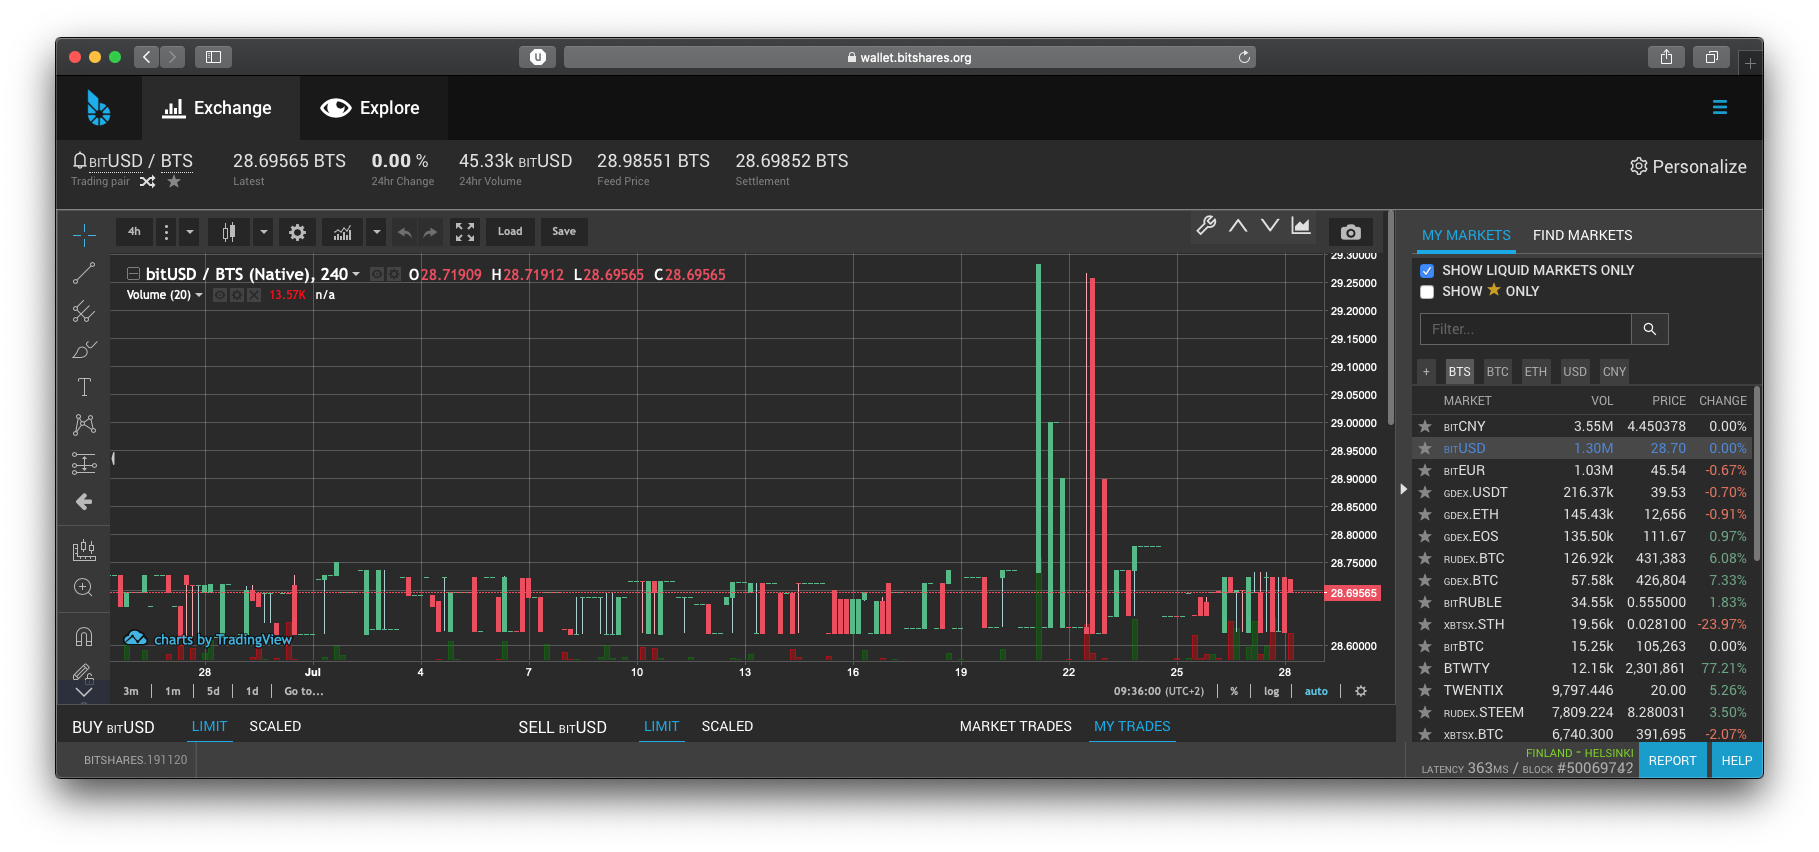
\includegraphics[width=\linewidth]{introduction/assets/bitshares}
	\caption{An online explorer provided by the BitShares DEX, showing recent and outstanding asset orders on the BitShares blockchain.}
	\label{fig:bitshares_explorer}
\end{figure}

\subsection{Decentralized Exchanges}
Blockchain technology is increasingly being used to build decentralized exchanges, also called \emph{DEXes}, to trade cryptocurrencies.
DEXes enable direct peer-to-peer trading without a market operator.
The first generation of DEXes limits trading to assets residing on the same blockchain.
On these DEXes, users can issue custom assets, transfer assets to others, and trade assets with other users by publishing buy and sell orders on the blockchain.
These orders are then automatically matched by miners during the validation of new transactions.
As we will further elaborate in Section~\ref{sec:matchmaking}, order matchmaking can also proceed outside the blockchain to increase efficiency, e.g., AirSwap~\cite{swap}.
Notable examples include Waves and BitShares which have accumulated a market capitalization of \$168 million and \$71 million dollars respectively at the time of writing.\footnote{https://coinmarketcap.com}
Figure~\ref{fig:bitshares_explorer} shows an online explorer of the BitShares blockchain, showing recent and outstanding asset orders.\footnote{https://wallet.bitshares.org}

We identify four advantages of DEXes over centralized cryptocurrency exchanges.
First, DEXes enhance security during the trading process; a trade is usually an atomic operation, and there is minimal risk of losing funds.
Second, users themselves remain in control of their funds when trading on a DEX and do not have to transfer ownership of their assets to the market operator.
Third, the transaction fees associated with trading on a DEX are usually lower compared to a centralized exchange since there is no profit-driven intermediary.
Forth, DEXes allow users to remain anonymous, whereas centralized exchanges often require the validation of one's identity.

Despite these advantages, many DEXes currently suffer from low liquidity and trading volume, making them less attractive for long-term trading.
Furthermore, their transaction throughput depends on the consensus model used by the underlying blockchain, which might make them unsuitable for bulk trading.
Finally, as DEXes are a relatively new technology, the user experience for traders can be perceived as overwhelming, in contrast to traditional exchanges which often provide a user-friendly trading interface.

\section{Disintermediation in Markets}
The popularity of electronic commerce has resulted in much interest to act as middlemen between buyers and sellers to benefit from their interactions~\cite{clark1999electronic}.
In many electronic markets, the role of matching buyers and sellers, and facilitating transactions is performed by a middlemen~\cite{bakos1998emerging}.
A well-known example is PayPal~\cite{paypal}, a payment service provider offering settlement services to customers buying goods from merchants.
PayPal not only process payments but it also acts as arbitrator when there a dispute between a buyer and seller arises.
The services of \emph{trusted intermediaries} such as PayPal is at the core of electronic market and ensures that a trade between a buyer and seller who might not necessarily trust each other proceeds without disputes.

Blockchain technology, and Bitcoin in particular, has challenged the need for trusted intermediaries.
In traditional payment systems, a financial institution acts as intermediary and handles payment between different (possibly foreign) banks.
Bitcoin has demonstrated that a decentralized system without financial institutions can be built, by leveraging cryptographic techniques.
Since the introduction of Bitcoin, there has been much effort by both industry and academia to critically look at the necessity of trusted intermediaries, and potentially replace them with another mechanism, e.g., smart contracts~\cite{lande2018sok}.
This process is also called \emph{disintermediation}.
Disintermediation usually lowers costs, since trusted intermediaries charge the involved traders for their services.
The process of disintermediation is tangential to the concept of decentralization (see Section X).
In particular, disintermediation requires decentralization as its foundation~\cite{guo2016blockchain}.

Disintermediation is a concept that pre-dates blockchain technology.
The Internet enabled quicker and convenient access to information, therefore opening opportunities to replace traditional broker agents~\cite{wigand2020whatever}.
A clear example of disintermediation can be found in the publishing market~\cite{giaglis1999disintermediation}.
Information technology enables book buyers to quickly place their order and authors to only print their books when there is actual demand.
This is also called printing-on-demand and removes the retailer from the traditional supply chain.

In many scenarios, it has been proven to be possible to disintermediate from a technical perspective.
Disintermediation is not always possible, nor desired.
However, in many scenarios there is a need to safeguard certain processes by intermediaries, in particular when considering the financial sector.
One might argue that electronic market require at least some intermediary to act as mediator between buyer and sellers if transactions are not atomic.
From a regulatory perspective, an intermediary can be required by law, e.g., when there is a need to verify the identify of new or existing business relations (this is also known as Know-your-Customer).

As also pointed out by other researchers, we argue that it is not likely that electronic markets will be fully disintermediated soon~\cite{zamani2018little}.
Rather than complete disintermediation, it is more likely that the role of existing intermediaries will be transformed.
For instance, financial institutions are currently exploring how distributed ledger technology can make their existing settlement services more efficient and reliable.
Perhaps the most influential solution, Corda, is currently being deployed by R3, a consortium consisting world's leading financial institutions~\cite{brown2016introducing}.
Another example is Ripple~\cite{armknecht2015ripple}, a credit network that is aimed to eventually replace the SWIFT payment infrastructure.
In practice, these solutions are not fully disintermediated since payments will still be processed by nodes operated by the involved financial institutions.


\section{Blockchain-based Marketplaces}
Given our definitions of decentralization and disintermediation in the context of electronic marketplaces, we now look how these concepts align with blockchain-based marketplaces.
Blockchain technology holds the promise to transform the market processes that currently require a trusted intermediary, e.g., when making payments to other peers.
It is important to clearly define what a blockchain-based marketplace means in the context of this work.
There is much confusion around the concept of blockchain-based marketplaces.
For example, the OpenBazaar market does not store its listings on a blockchain ledger but uses cryptocurrencies for peer-to-peer payments between merchants and customers.
In this work, \emph{a blockchain-based marketplace is a digital platform that leverages blockchain technology to carry out one or more of its critical operations}.

To better understand how this technology connects to existing market components, we describe the required components of blockchain-based marketplaces.
Figure~\ref{fig:electronic_markets} shows a decomposition of blockchain-based marketplaces.
This figure is the result of our literature survey where we have assessed both published and unpublished work on electronic marketplaces that use blockchain technology.
In general, we identify the following five mechanisms commonly used in blockchain-based marketplaces: \emph{matchmaking}, \emph{knowledge discovery}, \emph{settlement}, \emph{dispute resolution} and \emph{on-boarding}.
For each mechanism, we list approaches commonly found in the considered problem domain.
We now further discuss each identified mechanism. % the required components of blockchain-based marketplaces.

\begin{figure}[t]
	\centering
	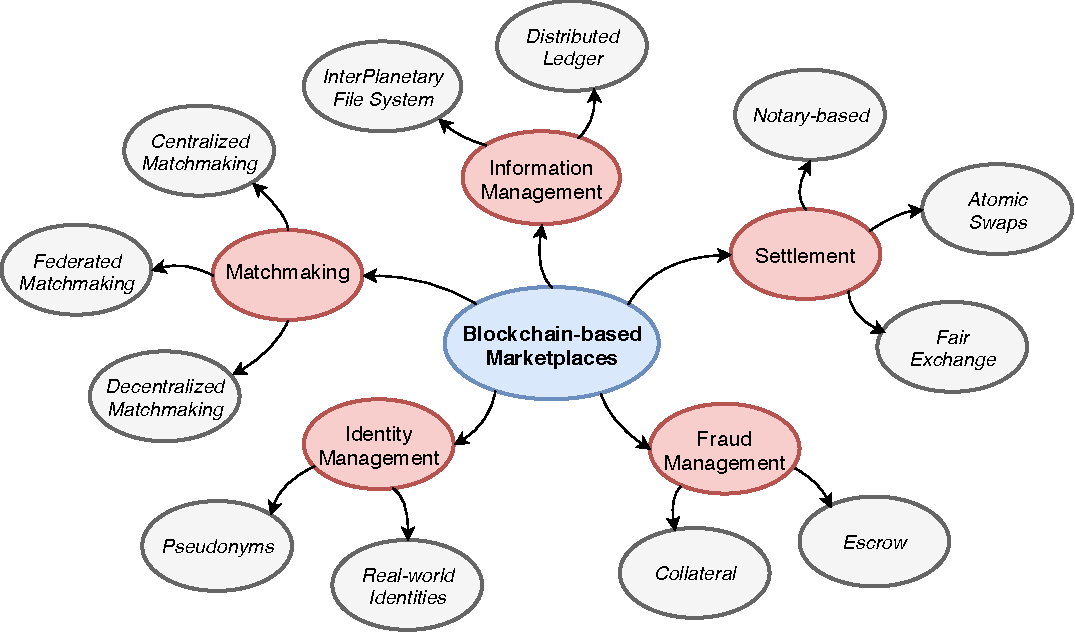
\includegraphics[width=\linewidth]{introduction/assets/decomposition}
	\caption{A decomposition of electronic marketplaces in four different components. Each component is further decomposed in approaches if applicable.}
	\label{fig:electronic_markets}
\end{figure}

\subsection{Knowledge Discovery}
Electronic marketplaces in general require a knowledge discovery mechanisms for market actors to enable value exchange.
Market knowledge includes pricing and product information, and details of past transactions.
Traditional electronic marketplaces usually store this information on centralized servers, deployed and managed by the market authority.
A key advantage of this approach for market operators is that these servers are relatively easy to setup and enable fast access to market information by participants.
Blockchain-based marketplaces usually avoid the storage of market information in a single location.
Therefore, market participants are dependent on others to retrieve the latest market state.

\subsubsection{Distributed Ledger}
A common approach for blockchain-based marketplaces is to store all available information on a distributed ledger.
This is, for example, the approach taken by DEXes like BitShares and Waves.
All market interactions are stored within tamper-proof transactions on a distributed ledger secured with global consensus.
Trades are either explicitly recorded in transactions, or can be derived from prior transactions.
Users wishing to get the latest market state are required to synchronize with the full distributed ledger from the network.
Since the distributed ledger might contain millions of transactions, some platform have setup a few \emph{full nodes} that remain synchronized in the network.
These full nodes offer an API that users can query to quickly retrieve market information.

\subsubsection{Order book}
A common market type is a financial exchange where financial instruments like currencies or bonds are being traded.
The buy and sell orders in these markets are usually bundled in an \emph{order book}.
An order book lists the specific assets or services that are being bought or sold within a market.
It provides traders with a convenient view on the current supply and demand.
Depending on the market and assets being traded, the order book sometimes reveals the identity of a trader behind an open order, or their reputation scores (for instance, Airbnb shows the reputation of hosts).
When presenting an order book to traders, ask and bid orders are usually sorted, i.e. based on their price.
For orders with a price, ask orders are sorted ascending on price in the order book and bid orders descending on price (the best orders are presented first).
%Market orders rarely end up in the order book as open order, since they are often fulfilled instantly.
%A defining metric used by traders is the difference between the price of the highest ask order and the price of the lowest bid order, also called the \emph{bid-ask spread}.
%For the order book shown in Figure \ref{fig:order_book}, the bid-ask spread is \$149.57 - \$149.54 = \$0.03.
%This metric also indicates market liquidity, the degree to which assets can be quickly bought or sold.
%A liquid market is often characterized by a low bid-ask spread.
The set of all ask or bid orders at a specific price is called a \emph{price level}.

\subsection{Settlement}
TODO

\subsubsection{Custodial}
A common approach to exchange blockchain-based assets is by using the services of a trusted intermediary.
A trade using a trusted intermediary completes as follows: two parties that agree on a trade transfer the assets for sale to one of the wallets owned by the trusted intermediary.
When this intermediary has received both assets, it finishes the exchange by transferring the appropriate assets to the other party.
In this approach, the trusted intermediary holds (temporary) ownership of the assets to be traded.
Relying on a trusted intermediary removes counterparty risk for the trading parties, but it requires both parties to have faith that the intermediary does not default or compromise their assets.

Trade through a trusted intermediary can facilitate value exchange between an extensive range of different blockchains, as long as the intermediary maintains wallets on the involved blockchains and can issue transactions in these systems to transfer the assets.
This is usually not an issue in permissionless blockchains since anyone can create accounts or wallets by generating a new cryptographic key pair.
Centralized cryptocurrency exchanges often facilitate asset trading across numerous permissionless blockchains.
Some cryptocurrency exchanges process transactions worth millions of dollars in total daily.\footnote{See https://coinmarketcap.com/rankings/exchanges}
In a permissioned blockchain environment, however, a trusted intermediary coordinating an asset exchange requires explicit approval from the operator to read and write transactions on the involved distributed ledgers.
Allowing new parties in a permissioned blockchain might be undesirable by operators since it introduces additional legal and operational risks.

\subsubsection{Atomic Swaps}
The \emph{atomic swap} is a distributed coordination task that allows asset exchange between different blockchains, without need for a trusted intermediary~\cite{herlihy2018atomic}.
Atomic swaps enable two parties to exchange blockchain-based assets with atomic guarantees: the asset exchange either completes or fails for both parties at any given time.
We now explain the involved operations during an atomic swap between the public Bitcoin and Ethereum blockchains.
Figure~\ref{fig:atomic_swap} visualizes the steps of an atomic swap between Alice and Bob, where Alice sells her Bitcoin in return for Ether (the native token of the Ethereum blockchain).
First, Alice generates a random secret $ s $ and computes $ H(s) $, where $ H(\cdot) $ denotes a hash function.
She then submits a hash-locked transaction, indicated by $ T_a(H(s)) $ (step \circled{1}), to the Bitcoin blockchain that transfers her Bitcoin to Bob's wallet address.
A hash-locked transaction is only executed when the secret $ s $ is provided to it.
Alice now sends $ H(s) $ to Bob (step \circled{2}).
Bob then submits a transaction $ T_b(H(s)) $ with the same hash lock to the Ethereum blockchain, transferring his Ethereum to the account of Alice (step \circled{3}).
Alice is now able to claim the assets held in custody by $ T_b(H(s)) $ (since she knows the value of $ s $), which in turn reveals $ s $ to Bob (step \circled{4}).
Bob now completes the swap by submitting $ s $ to the $ T_a(H(s)) $ transaction on the Bitcoin blockchain, which unlocks the assets in $ T_a(H(s)) $ (step \circled{5}).
To prevent the situation where assets are locked indefinitely if Alice refuses to reveal $ s $, Alice and Bob submit two additional time-locked transactions to ensure that assets in $ T_a(H(s)) $, respectively $ T_b(H(s)) $, can be claimed after some time $ t_1 $, respectively $ t_2 $.
To address the situation where Alice claims the assets in both $ T_a(H(s)) $ and $ T_b(H(s)) $, it must hold that $ t_1 > t_2 $.
These hash- and time-based agreements, also called Hashed Timelock Contracts (HTLCs), thus ensure trust-less, atomic asset exchange between trading parties, assuming that they claim the assets before the time-lock expires.
Atomic swaps eliminate the risk of losing assets to an adversarial trader while trading.
The HTLC atomic swap requires a total of four transactions.

\subsubsection{Notary-based}
Notary schemes are another solution for asset exchange where approval by a group of credible nodes (notaries) is required to perform some operation.
Notary schemes aim to partially alleviate the trust issues arising when relying on a single trusted intermediary through the approval by a group of semi-trusted notaries instead.
These notaries reach consensus on the occurrence of particular events, e.g., on the inclusion of a transaction on a distributed ledger.
Compared to an asset exchange through a trusted intermediary, notary schemes assume a weaker trust model and can often withstand adversarial behavior of a fraction of the notaries.

The Interledger project, introduced by Ripple, is the most advanced approach in this direction~\cite{thomas2015protocol}.
Interledger proposes a notary-based protocol to conduct payments across different ledgers.
In atomic mode, these payments are realized through atomic swaps and are coordinated by a different group of notaries for every involved blockchain.
Interledger uses payment paths where additional intermediate platforms and their notaries are used to exchange assets between ledgers that do not have a direct connection.
Interledger also supports bidirectional asset exchange but is vulnerable to a fraction of notaries colluding with one of the trading parties.
External coordination is avoided in universal mode, which relies on incentives for participants to behave honestly and not to commit fraud.
The Hyperledger Quilt project provides a Java implementation of the Interledger protocol for permissioned blockchains~\cite{hyperledgerquilt}.

\subsubsection{Fair Exchange}
TODO

\begin{figure*}[t]
	\centering
	\begin{subfigure}[t]{.33\textwidth}
		\centering
		\captionsetup{width=.9\linewidth}
		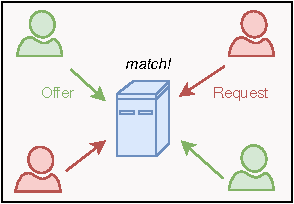
\includegraphics[width=.9\linewidth]{introduction/assets/centralized_matchmaking}
		\caption{\emph{Centralized matchmaking}: new orders are always sent to a single matchmaker, usually a centralized system (server).}
		\label{fig:centralized_matchmaking}
	\end{subfigure}%
	\begin{subfigure}[t]{.33\textwidth}
		\centering
		\captionsetup{width=.9\linewidth}
		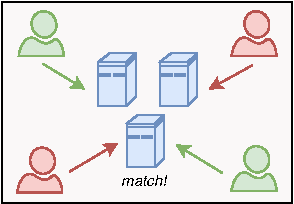
\includegraphics[width=.9\linewidth]{introduction/assets/federated_matchmaking}
		\caption{\emph{Federated matchmaking}: new orders are sent to one of the available matchmakers in the network.}
		\label{fig:federated_matchmaking}
	\end{subfigure}%
	\begin{subfigure}[t]{.33\textwidth}
		\centering
		\captionsetup{width=.9\linewidth}
		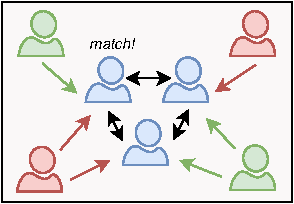
\includegraphics[width=.9\linewidth]{introduction/assets/decentralized_matchmaking}
		\caption{\emph{Decentralized matchmaking} (our proposal): new orders are sent to multiple matchmakers and shared between them.}
		\label{fig:decentralized_matchmaking}
	\end{subfigure}
	\caption{Three models for order matching. Traders create offers and requests (colored green and red respectively), which are matched by matchmakers (depicted in blue).}
	\label{fig:matching_models}
\end{figure*}

\subsection{Order Matchmaking}
\label{sec:matchmaking}
Automatically \emph{matching} customers is a prerequisite for online trade and therefore essential for electronic marketplaces.
Matchmaking is defined as the process of mediating supply and demand in markets, based on profile information~\cite{Veit:2003fs}\footnote{In multi-agent systems, a matchmaker is considered as an entity that only aggregates offers. Brokers aggregate both offers and requests. We will use the term matchmaker in this paper since we found it to be more common in related work.}.
Notable examples are matching idle agents to incoming jobs or matching suppliers of specific assets to consumers who are interested in buying these assets.
Inefficient matchmaking between participants decreases overall market efficiency and customer satisfaction~\cite{Wu2015TheM}.
%For example, in a ride-hailing marketplace like Uber, it is key to match nearby drivers and passengers in a timely and efficient manner.
For instance, prolonged suboptimal matching by ride-hailing marketplaces such as Uber increases the waiting time for passengers and results in drivers having to traverse a greater distance to pick up their customers.
%Similarly, inefficient matching of available computer resources to customers by cloud providers could violate service-level agreements, resulting in customer loss and reputational damage.

In this section, we review different approaches to order matchmaking in electronic markets.
Matchmaking depends on the individual constraints and preferences of market participants.
In most electronic markets, a participant includes this information in an \emph{order} that indicates their intention to buy and sell assets, resources, or services~\cite{Veit:2003fs}.
This order is then submitted to a matchmaker.
In general, economic literature distinguishes between two types of orders: \emph{asks}, created by traders offering a specific asset, service, or resource, and \emph{bids}, created by interested buyers.
%Each order can have multiple attributes attached, e.g., a price or a location.
The main objective of a matchmaker is a quick and effective mediation between incoming offers and requests, based on constraints and preferences included in each order.

We identify three different approaches to order matchmaking, depicted in Figure~\ref{fig:matching_models}.
With \emph{centralized matchmaking} (Figure~\ref{fig:centralized_matchmaking}), traders submit their asks and bids to a single server.
With \emph{federated matchmaking} (Figure~\ref{fig:federated_matchmaking}), traders submit a new order to one of the servers of their choice.
Finally, in \emph{decentralized matchmaking} (Figure~\ref{fig:decentralized_matchmaking}), traders submit their orders to one or more matchmakers.
We further elaborate on each matchmaking model.

\subsubsection{Centralized Matchmaking}
Figure~\ref{fig:centralized_matchmaking} visualizes the centralized matchmaking model, which is the most common approach to match orders.
Traders send new offers and requests to a dedicated matchmaker, usually a centralized system (server).
This model is widely adopted by commercialized marketplaces such as stock exchanges or peer-to-peer service markets like Uber.
A matchmaker bundles open orders in a local data structure known as an \emph{order book}.
The order book stores all active asks and bids, and provide traders a convenient view on the current supply and demand.
A new incoming ask or bid is then matched with other bids and asks, respectively, using a \emph{matching policy}.
The most common matching policy used in cryptocurrency exchanges is the \emph{price-time} strategy, where orders are first matched based on the price, and then on their order creation time (older orders are prioritized).
The order book is often optimized for fast order lookup and matching within a specific trading domain.

The EtherDelta decentralized exchange is one of the first DEXes that adopt the centralized matchmaking model~\cite{Anonymous:brZbAflS}.
EtherDelta maintains a single server that stores an order book with all active orders.
Traders can browse the order book and trade against orders in the order book.
The trades are finalized on the blockchain, and the order is then removed from the EtherDelta order book.\todo{custodial vs non-custodial}
The IDEX exchange also deploys a centralized server but automatically matches orders submitted by makers and takers~\cite{AuroraLabs:B4jmyRY8}.
Specifically, traders lock their assets in the IDEX smart contract and submit their order to the IDEX server, which checks its validity.
The order is then executed by the Ethereum smart contract and the order book is updated according to the executed trade.

A main advantage is that the centralized matchmaking model with a single server is relatively straightforward to implement, since no communication or order book synchronization is required.
Also, since all orders are stored and matched by single matchmaker, orders are processed based on full market knowledge.
The identity behind each order is only known to the market operator, therefore protecting the privacy of individual traders.

Unfortunately, the emergence of electronic trading in general gave rise to fairness, transparency and manipulation issues during the matchmaking process~\cite{Mavroudis:2019iw}.
For example, the EtherDelta operator is able to censor specific orders.
Furthermore, information asymmetry between exchange operators and traders allows operators to front-run specific orders (see Section X\todo{x}).
The work of Mavroudis and Melton address fairness issues arising from the latency traders experience when submitting orders and gaining market information~\cite{Mavroudis:2019iw}.
They propose Libra, an order reordering matching policy that alleviates the effects of uneven delays by the market infrastructure.
Libra remains temporally fair, meaning that among all pairs of participants on it the probability that a slower participant succeeds in capturing a trading opportunity at the expense of a faster participant (who, responsive to the same stimulus, is also competing for the same opportunity) does not exceed 0.5.

From a systems perspective, centralized matchmaking has a low scalability compared to distributed solutions since the matchmaker becomes a bottleneck when more orders are created in the same time period.
Fault tolerance is another concern: if the single matchmaker becomes unavailable, e.g., due to infrastructure failures, incoming orders cannot be matched and all market activity stalls.

\subsubsection{Federated Matchmaking}
Figure \ref{fig:federated_matchmaking} illustrates an alternative model for order matching: federated matchmaking.
Instead of relying on a central matchmaker, multiple (independent) matchmakers individually maintain an order book.
The group of matchmakers can either be static (e.g., elected by a committee or a voting mechanism), or dynamic (e.g., each peer can opt-in to become a matchmaker).
A trader now submits new orders to their preferred matchmaker (for example, based on the reliability or trustworthiness of individual matchmakers).
The 0x and Swap protocols are notable examples of the federated matchmaking model and are discussed next.

%Blockchain-powered marketplaces based on the 0x and AirSwap protocols have adopted the federated matchmaking model~\cite{warren20170x}~\cite{oved2017swap}.
The 0x protocol uses off-chain order relaying and on-chain settlement, meaning that orders are created shared, and matched outside a blockchain.
A maker creates market liquidity in 0x by first selecting an available relayer.
Each relayer maintains an off-chain order book and charges a transaction fee for its services.
The maker then creates the order and specifies a fee which is given by the selected relayer.
Takers query the order book of relayers and if they intend to fulfill an order, they submit it to the Ethereum blockchain.
The Augur prediction market (see Section~\ref{sec:prediction_markets}) leverages the 0x protocol for order dissemination and matching.

The Swap protocol follows a similar off-chain matchmaking, on-chain settlement model~\cite{oved2017swap}.
In Swap, indexers aggregate trade intents created by market makers and takers.
The indexer informs takers when a matching trade intent has been found, upon which a peer-to-peer negotiation process starts between the matched maker and taker.
During this negotation process, a maker may contact an oracle to get a price suggestion.
When a maker and taker agree on a trade, the taker submits the agreement to an Ethereum smart contract, upon which the trade is executed and on-chain assets are exchanged.
We remark that both 0x and Swap are limited to trading Ethereum-based digital tokens and can therefore not be used for order processing of any blockchain-based asset.

The federated matchmaking model gives traders the opportunity to use the services of their preferred matchmaker.
Manipulative behaviour of one matchmaker then leads to the situation where traders select another, honest matchmaker.
Furthermore, unavailability of an individual matchmaker is less likely to stall all market activity since a trader can send their orders to another available matchmaker.
However, the order book is fragmented across different matchmakers, potentially leading to less market efficiency and liquidity, compared to matchmaking with an order book managed by a single entity.

\subsubsection{Decentralized Matchmaking}
%Scalability limitations, low fault tolerance, and uneven load balancing are inherent issues of centralized and federated matchmaking.
The \emph{decentralized matchmaking} model is depicted in Figure \ref{fig:decentralized_matchmaking}.
The main idea is that a single order is sent to multiple matchmakers simultaneously and matchmakers share their orders with other matchmakers (liquidity sharing).
We distinguish between on-chain and off-chain decentralized matchmaking.

\textbf{On-chain.}
We now discuss on-chain matchmaking approaches that either rely on a smart contract to match incoming orders, or embed the matchmaking logic in the transaction validation logic.
The Stellar protocol integrates DEX functionality that enables users to create buy and sell orders that trade assets native to the Stellar ledger~\cite{Lokhava:2019kd}.
These orders are created using specific transaction types, that are matched with existing, outstanding orders during inclusion of the transaction in the ledger.
The Stellar matching engine uses the price-time policy.
Similarly, the BitShares blockchain provides functionality to create orders at the protocol level~\cite{Schuh:CsvWDxUZ}.

The main advantage of on-chain matchmaking is tight integration with the blockchain platform; no external components such as a peer-to-peer overlay are needed to process orders.
Instead, all orders can simply be processed by the blockchain logic.
This also makes it more convenient for users to submit their orders.
On the other hand, since users likely need to pay transaction fees when creating new orders or when cancelling existing ones, trading in bulk can become a costly process.
Furthermore, blockchain-based order matching can be orders of magnitude slower compared to centralized matchmaking, due to security requirements.
Finally, on-chain matching protocols do not explicitly store the history of matches.
Therefore, the reconstruct the order book at a specific block height, one needs to process all transactions up to that point.

\textbf{Off-chain.}
To overcome transaction fees and slow transaction confirmation times, some platforms maintain a fully decentralized order book off-chain.
An example of off-chain decentralized matchmaking is the Loopring protocol, which builds a decentralized order sharing protocol~\cite{Wang:wt}.
Loopring is able to mix and match multiple orders in circular trade, also called order rings, therefore increasing liquidity.
New orders are sent to one or more relays in a mesh network.
Order rings are submitted to a smart contract, e.g., on Ethereum, where the trade is then executed.
Relayers can optionally share orders with other relayers to increase liquidity, however, the whitepaper lacks technical details on how this is achieved specifically.
Relayers take the margin between two matched orders, or can charge some fee.
% front-running in Loopring

The Republic Protocol builds a decentralized network of nodes that match orders without revealing any information about individual orders~\cite{Zhang:kGvi0me4}.
Specifically, it uses Shamir Secret Sharing to break down an order in multiple order fragments which are distributed through the network.
An Ethereum smart contract, called the Registrar, describes the network topology such that it is hard for an adversary to fully reconstruct an original order.
Nodes cooperate with other nodes to check if their order fragments match, by computing a zero-knowledge proof.
When two order fragment match, an atomic swap is initiated between the two traders (also see Section~\ref{sec:atomic_swap}).
Note that this prevents an individual from estimating the total liquidity in the network.

We identify two advantages of this model over centralized and federated matchmaking.
First, sharing orders between matchmakers can yield the same matching effectiveness compared to centralized matchmaking, depending on the order synchronization details. %since orders can be synchronized amongst matchmakers.
Second, decentralized matchmaking should show higher tolerance against failure of individual matchmakers.
However, this model increases bandwidth usage since orders are sent to multiple matchmakers.
Also, it might take longer before a new order is fulfilled in the case that it is sent to matchmakers that are unable to match this order immediately.

\subsection{Identity Management}
Identity management is a key component of any electronic market.
Traditional electronic marketplaces usually impose some form of identity validation before a user is allowed to engage in trade with other users.
In this situation, the digital identity is linked to real-world credentials, e.g., a passport.
Identity validation in electronic marketplaces has several purposes.
First, it adds accountability of ones actions within the market in case of a dispute between a buyer and seller.
Second, it prevents the situation where a user can easily re-enter the market under a different identity after having committed fraud.
Third, identity verification is often part of the regulatory compliance of market operators, as often required by anti-money laundering policies.
Most cryptocurrency exchanges managed by a central market authority require users to verify their identity before they can create buy or sell orders.

In stark contrast with traditional marketplaces, a key property of blockchain technology is the ability to join the network under a pseudonym, using a locally generated cryptological keypair.
In Bitcoin, for example, users can easily transfer Bitcoin to others using different digital identities.
This is even the preferred practice when one wants to retain anonymity in the Bitcoin network.
Similarly, many DEXes do not require identity verifications and allow traders to join the network under a pseudonym.

\subsection{Fraud Management}
Fraud is a key concern in electronic marketplaces.
A common type of fraud is \emph{counterparty fraud}, where a party does not fulfil its obligation towards the counterparty during trade settlement, e.g., by not delivering the promised assets or goods.
This kind of fraud is often resolved by the market operator, acting as arbitrator during the dispute resolution process.
Within blockchain-based marketplaces, counterparty fraud is often prevented since asset exchange is atomic: either all parties receive their assets or nothing happens.
This approach works when assets can be exchanged directly, e.g., on a blockchain-powered DEX.
Fraud management, however, is required when settlement depends on the actions by users.
We identify different approaches to manage fraud.

\subsubsection{Escrows}
TODO

\subsubsection{Collateral}
Some blockchain-based marketplaces require users to deposit collateral before trading.
This collateral is slashed when its depositor does not adhere to an agreement and therefore incentivise traders to follow the protocol.
The XClaim protocol relies on collateral deposits to enable asset trading between distinct blockchain ledgers.
When a participant deviates from the protocol, the collateral is slashed and wronged actors are reimbursed.

%\section{Problem Statement}
%The key issue is that decentralized applications that are using blockchain technology are often not scalable enough.

\section{Research Questions}
In this thesis, we mainly focus on \emph{knowledge discovery}, \emph{matchmaking} and \emph{settlement} in electronic markets.

The overarching research question of this thesis is as follows:\\\\
\emph{How can we improve matchmaking and settlement mechanisms in blockchain-based marketplaces?}\\\\
To answer our research question, we address the following key questions:

\textbf{[RQ1] What is the state-of-the-art in blockchain-based electronic trading and asset exchange?}
To provide an answer to our research question, it is required to build an understanding of state-of-the-art approaches to blockchain-based trading, and their shortcomings.
Even though there is much active research on blockchain-based decentralized exchanges and secure asset trading between heterogeneous blockchain platforms, the field lacks a systematic literature overview, an analysis of open challenges and suggestions for further research.

\textbf{[RQ2] How can we efficiently match market orders without centralized coordinator?}
The predominant approach to order matchmaking in electronic markets is by using a centralized server, owned by the market operator.
This approach, however, enables manipulation by the operator, resulting in an unfair system.
Blockchain-based matchmaking has the potential to address fairness issues but is by far not scalable enough for usage by many marketplaces.
We aim for an efficient matchmaking mechanism with fairness guarantees, not under the control of a single market operator.

\textbf{[RQ3] How can improve settlement durations of (international) payment infrastructures?}
A major problem of current banking systems is that the settlement duration of a payment between two different (international) banks is significant, often in the order of days.
Furthermore, these payments require significant transaction fees to cover back-office costs.
Blockchain technology holds the potential to improve the speed of (international) payment infrastructures, and potentially lead to a reduction of costs and lower transaction fees.

\textbf{[RQ4] How can we exchange assets managed by different blockchains?}
Decentralized exchanges (DEXes) is a new type of decentralized application where digital assets are issued and traded on a blockchain.
Compared to centralized exchanges, DEXes take a non-custodial approach where users manage these assets themselves.
The main issue, however, is that the assets on a specific DEX are locked to a single blockchain; trade between different DEXes is either impossible or slow.
The question is how to address these issues and enable fast asset trading between different exchanges.

\textbf{[RQ5] How can we apply blockchain technology to improve software crowdsourcing markets?}
The engineering of blockchain-based applications such as exchanges is a challenging task and requires engineers with appropriate qualifications.
Crowdsourcing is a relatively new model for software development, where an open call is made for the documentation, design, coding, and testing of software.
Recent research proposes to leverage blockchain technology
Applying accountability and fraud detection could improve the software crowdsourcing process.

\begin{table*}[t]
	\small
	\centering
	\begin{tabular}{ |c|c|c|c| }
		\hline
		\textbf{Chapter} & \textbf{Mechanism} & \textbf{DAS5 experiments?} & \textbf{Deployment?} \\ \hline
		2 & TrustChain & yes & yes, integration in Tribler \\ \hline
		3 & MATCH & yes & yes, integration in Tribler \\ \hline
		4 & XChange & yes & yes, integration in Tribler \\ \hline
		5 & Internet-of-Money & yes & in-house testing \\ \hline
		6 & DevID & no & user trial \\ \hline
	\end{tabular}
	\caption{An overview of research methods for each mechanism introduced in this thesis.}
	\label{table:research_methodology}
\end{table*}

\section{Research and Engineering Methodology}
Blockchain technology is a relatively new and immature field.
We identify two fundamentally different approaches to the adopted research methodology in this field.
On one hand, published blockchain research in systems-oriented conferences follow an experimental methodology where the performance of the proposed mechanism is systematically evaluated using a comprehensive set of experiments and benchmarks.
On the other hand, there is a vast body of research on the security aspects of distributed ledgers.
This kind of research tend to follow a more theoretical approach through the use of formal proofs or small-scale protocol simulations.

In this work, we adopt an experimental-driven approach where we answer each research question by designing, implementing and evaluating a system or mechanism.
We then systematically evaluate the appropriate properties of each mechanism, and if feasible, we deploy our mechanisms to users to gather real-world results.
For all of our proposed mechanisms, we aspire a practical solution, ready for deployment and usable by real users.

Distributed systems can be complex software implementations with many components that work together.
Specifying the scope of a system is a non-trivial challenge and failing to implement clear system boundaries can result in numerous performance bottlenecks and degradation of user experience when such a system is deployed.
To this end, during the design of each mechanism we specify the boundaries of each system and state what we consider out of scope.
We aim to focus on the core functionality of each mechanism.

Table~\ref{table:research_methodology} specifies for each mechanism whether we present a set of DAS5 experiments and/or whether we have conducted a real-world deployment.
Except for DevID, we evaluate each component using a comprehensive set of experiments that have been conducted on our DAS5 nation-wide compute cluster.

Driven by our focus on practicality, we have deployed each mechanism proposed in this thesis, either to a small group of users or with an integration in Tribler.
Tribler is our academic testbed and offers decentralized, anonymous file-sharing capabilities.
Tribler has been downloaded by over 1.5 million users and enables us to test our ideas in a geo-distributed, real-world environment.
We have evaluated TrustChain, for example, in the context of our anonymous file-sharing overlay to address free-riding behaviour.
This longitudinal deployment allowed us to incrementally improve our software and refine our ideas.
Due to legal considerations, we have been unable to provide an open-source implementation of the Internet-of-Money mechanism.

We ensure that each mechanism is tested.
Even though this is uncommon practice for research projects, we believe that a proper engineering methodology adds credibility to the presented mechanisms, helps reproducibility and is instrumental in getting a system ready for deployment.

% simplicity?

%We believe this experimental research methodology is suitable for two reasons.
%First, it allows us to evaluate our ideas in an environment that closely resembles a real-world environment.
%Second, it directly leads to a software implementation that can be used by academia or industry.
%All developed software artefacts are available on our GitHub repository and contain unit tests to verify functional correctness.

% existing research does X

% but we do Y!

\begin{figure}[t]
	\centering
	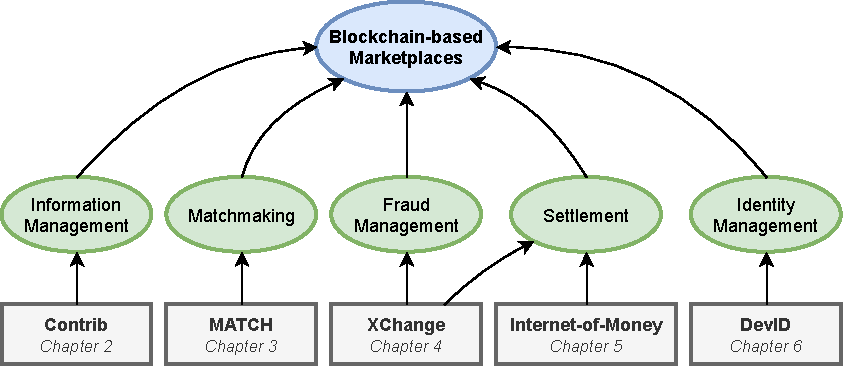
\includegraphics[width=\linewidth]{introduction/assets/thesis_overview}
	\caption{The five mechanisms presented in this work (depicted in grey), in the context of blockchain-based marketplaces and their components.}
	\label{fig:thesis_overview}
\end{figure}

\section{Contributions and Thesis Outline}
After establishing the required background on decentralized applications and distributed ledger technology, Chapter \todo{X} highlights scalability limitations of state-of-the-art blockchain ledgers.
Next, in Chapter \todo{X}, we design, implement and evaluate TrustChain: a scalable blockchain ledger that is based on fraud \emph{detection} instead of fraud \emph{prevention}.
In Chapters \todo{X to Y}, we apply accountability primitives and fraud detection techniques in three well-established domains: financial transactions, two-sided marketplaces, and identity.
Specifically, we make the following contributions in each chapter:\\

\textbf{[Chapter 2] SoK: Electronic Markets in the Age of Blockchain.} (Work in progress)
In this chapter, we answer RQ2 and provide an extensive overview of existing approaches for online trade in the age of blockchain.\\

\todo{Work in progress}\\

\textbf{[Chapter 3] MATCH: Accountable and Generic Matchmaking for Decentralized Applications.}
In this chapter, we partially address RQ4 and focus on matchmaking, the process of bringing market participants together based on individual preferences.
Matchmaking is a cardinal, yet overlooked prerequisite for a fully decentralized exchange.
Although numerous companies have deployed infrastructure for matchmaking, there is currently no solution that can be deployed within different trading domains.
We present MATCH, a middleware for generic order matching.
Since MATCH is agnostic about order specifications, the resulting system is highly flexible and reusable.
In this work, we first present an alternative approach to order matching, named \emph{decentralized matchmaking}.
The main idea is that new orders are disseminated to multiple matchmakers simultaneously and shared between matchmakers.
We then design and implement a novel matching protocol and a middleware with full support for both existing matchmaking paradigms and decentralized matchmaking.
Finally, we extensively evaluate desired system properties of MATCH under a real-world ride-hailing and asset trading workload.
Our main finding is that decentralized matchmaking exhibits superior fault tolerance and load balancing, at the cost of moderately increased bandwidth usage and order completion time.
This chapter is based on the following publication:

\todo{UNDER REVIEW}\\

\textbf{[Chapter 4] XChange: A Scalable Asset Marketplace based on Accountability.}
In this chapter, we answer RQ4 and introduce XChange, an asset marketplace based on accountability guarantees.
There is an increasing need for a generic mechanism to trade assets across isolated platforms, as more industries rely on the digital management of their physical resources using Internet-of-Things devices.
To date, there is no such mechanism without dependency on a trusted third party.
We address this shortcoming and present XChange, a blockchain-based mechanism for generic asset trading.
Unlike existing asset trading marketplaces, we decouple trade management and the actual exchange of assets.
XChange enables the trustworthy trade of \emph{any} digital asset.
We describe a generic trading protocol that establishes trade between individuals and accounts market activity on any distributed ledger.
We prove with a theoretical analysis that the effectiveness of fraud conducted by adversarial parties is limited.
Furthermore, we devise a novel market architecture, composed of all required components for a decentralized asset marketplace.
We implement the XChange mechanism and conduct real-world evaluations.
To account market activity in a tamper-proof manner, we use an existing scalable blockchain ledger, TrustChain.
By deploying XChange on multiple low-resource devices, we show that a full trade can be completed within 500 milliseconds.
To analyze the scalability and bandwidth usage, we conduct further experiments on our compute cluster and deploy up to 500 XChange instances.
Our main finding is that the throughput of XChange, in terms of trades per second, scales linearly with the network size.
This chapter is based on the following publication:

\todo{UNDER REVIEW}\\

\textbf{[Chapter 5] Internet-of-Money: Applying Accountability to Enable Real-time International Money Transfers.}
In this chapter, we answer RQ3 and explore a new stage in the evolution of digital trust, trusting strangers with your money.
We address the challenging problem of giving money to others and relying on them to forward it.
To identity fraud, we account money transfers between interacting strangers.
This work represents a small step towards a generic infrastructure for trust, moving beyond proven, single-vendor platforms like eBay, Uber and AirBnb.
Expanding upon trust relations, we designed, implemented and evaluated an overlay network: \emph{Internet-of-Money}.
Internet-of-Money is capable of real-time money transfers to different banks by routing funds through individuals (\emph{money routers}).
This removes the need for central banks to handle a payment.
Our network reduces traditional payment durations from a day or even a few days in weekends, to mere seconds.
%Internet-of-Money is fully decentralized, privacy-preserving and highly scalable.
With real-world experimentations, we prove that Internet-of-Money enables fast money forwarding.
We show that our overlay network is capable of discovering a majority of available money routers within a minute.
Finally, we demonstrate how profit of cheating routers is limited and that misbehaviour is punished.
This chapter is based on the following publication:

Martijn de Vos and Johan Pouwelse, \enquote{Real-time Money Routing by Trusting Strangers with your Funds}, \emph{IFIP Networking, 2018.}\\

\textbf{[Chapter 6] DevID: Blockchain-based Portfolios for Software Developers.}
In this chapter, we answer RQ5.
Decentralized applications, also known as dApps, are the new paradigm for writing business-critical software.
Recruiting developers with appropriate qualifications and skills for this activity is key, yet challenging.
The main problem is that the portfolio of developers is usually scattered across centralized platforms like GitHub and LinkedIn, and vendor locked.
This can result in an incomplete impression of their capabilities.
We address this problem and introduce \emph{DevID}, a blockchain-based portfolio for developers.
Over time, this portfolio enables developers to build up a trustworthy collection of records that showcase their capabilities and expertise.
They can import data assets from third parties into a unified DevID portfolio, add projects and skills, and receive endorsements.
All portfolio records are stored on a scalable distributed ledger and owned by developers themselves.
The essential idea is to exploit the tamper-proof property of the blockchain while providing durable storage.
To demonstrate the practical value of DevID, we build the competition-based platform, \emph{dAppCoder}, for the development of decentralized applications.
On dAppCoder clients are able to submit their ideas and developers can find work.
dAppCoder utilizes DevID portfolios to match these clients and developers.
We fully implement our ideas and conduct a deployment trial.
Our trial demonstrates that DevID is efficient at storing portfolio records.
This chapter is based on the following publication:

Martijn de Vos, Mitchell Olsthoorn and Johan Pouwelse, \enquote{DevID: Blockchain-based Portfolios for Software Developers}, \emph{IEEE International Conference on Decentralized Applications and Infrastructures (DAPPCON'19)}\\

\textbf{[Chapter 7] Conclusion.} We will end this thesis with the conclusion, a summary of the lessons learned, and suggestions for further work.

%\begin{figure}[t]
%	\centering
%	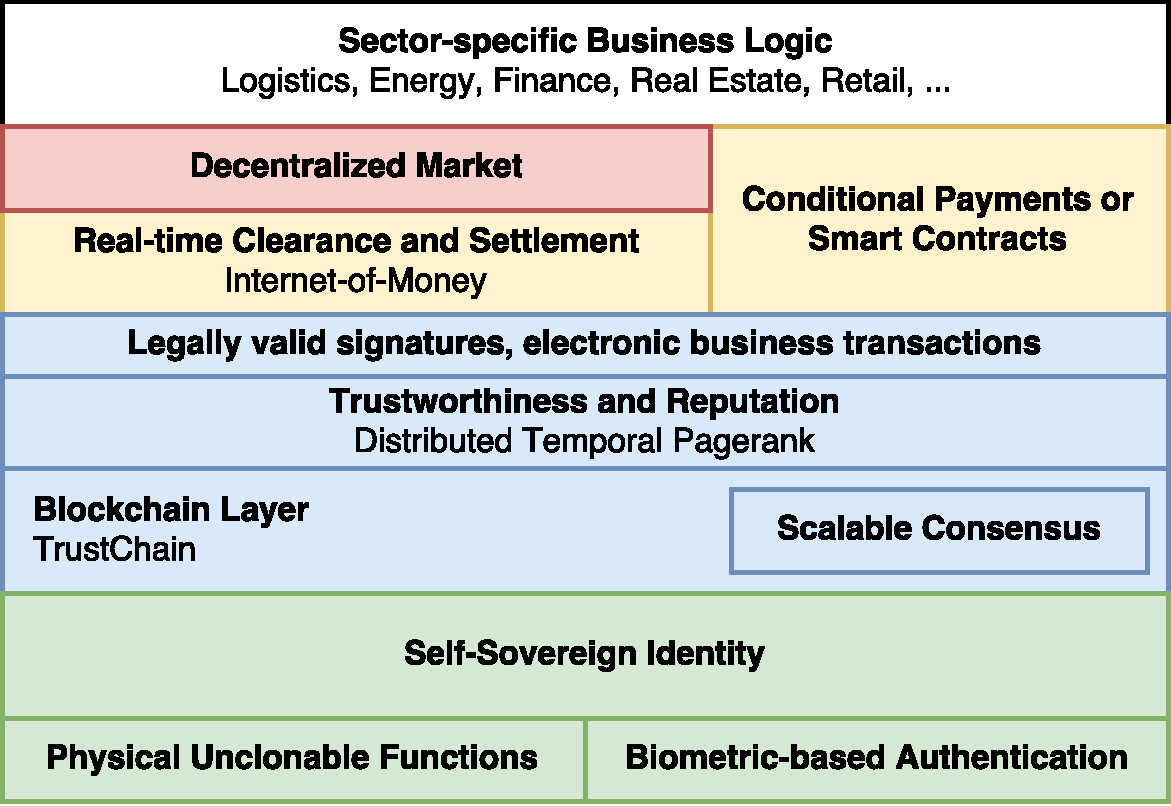
\includegraphics[width=.7\linewidth]{introduction/assets/tech_stack}
%	\caption{An overview of the research conducted at the Delft Blockchain Lab.}
%	\label{fig:dbl_tech_stack}
%\end{figure}

%\section{About the Delft Blockchain Lab}
%The Delft Blockchain lab is Delft's initiative for research, education and training in blockchain technology and trust on the Internet.
%Figure~\ref{fig:dbl_tech_stack} outlines the research directions of the Delft Blockchain Lab, ranging from low-level primitives like biometric-based authentication to sector-specific business logic.
%At the lowest layers (depicted in green), we build, deploy and evaluate new solutions for managing ones identity in the physical world and on the Internet.
%These solutions include biometric-based authentication and physical unclonable functions, a method to securely store a private key.
%A part of our ongoing research includes a self-sovereign identity solution that is currently being tested and deployed in the Netherlands.

%Our research effort around distributed ledger technology includes scalable consensus algorithms and Sybil-resistant reputation mechanisms.
%The TrustChain distributed ledger is presented in Chapter X.
%The other components of this thesis are mostly focussed on the research directions that are coloured yellow and red in Figure~\ref{fig:dbl_tech_stack}.
%For a detailed outline of our research efforts, we refer the reader to our published vision paper.

%\newpage

%\bibliographystyle{unsrt}
%\bibliography{introduction}
\chapter{Conclusions}
\label{conclusion}

In this thesis, we have introduced five novel mechanisms to decentralize and disintermediate all aspects of blockchain-based marketplaces.
Using our universal \TrustChain{} accounting mechanism, market information can securely be stored in a decentralized manner by peers themselves.
With our decentralized MATCH middleware, participants do not have to rely on a centralized matchmaker to match their orders in peer-to-peer markets.
Our XChange trading mechanism enables asset trading between permissioned blockchains without any requirement for a trusted third party that performs settlement.
The decentralized Internet-of-Money overlay enables fast and international money transfers without settlement by a central bank.
Finally, software developers using DevID can build self-hosted, durable portfolios without their data being managed by a central party can and showcase these portfolios on the decentralized crowdsourcing platform DAppCoder.

\section{Conclusions}
The main conclusions of this thesis are as follows:

\begin{enumerate}
	\item In Chapter~\ref{chapter:trustchain}, we have built \TrustChain{}, a universal accounting mechanism.
	With a two-year deployment trial of \TrustChain{} in our peer-to-peer application \Tribler{}, we have successfully addressed free-riding behaviour in our Tor-like overlay.
	Our \TrustChain{} mechanism is highly suitable for accounting data within different application domains that can tolerate fraud to remain undetected for a short period.
	In this thesis, we have leveraged the accounting capabilities of \TrustChain{} to store data elements in the XChange (Chapter~\ref{chapter:xchange}), Internet-of-Money (Chapter~\ref{chapter:iom}) and dAppCoder/DevID (Chapter~\ref{chapter:devid}) mechanisms.
	
	\item Our decentralized MATCH middleware, presented in Chapter~\ref{chapter:match}, is highly resilient against manipulation during order matchmaking.
	This manipulation is a significant concern in peer-to-peer markets under central ownership.
	MATCH performs high-quality matchmaking and does so with bandwidth and memory overhead orders of magnitude lower compared to matchmaking on a blockchain.
	We are the first to experiment with a fair and decentralized alternative to the Uber ride-hailing market.
	
	\item In Chapter~\ref{chapter:xchange}, we have presented a novel approach for asset trading between permissioned blockchains.
	Compared to existing trading approaches that either require third party intervention or modifications to deployed blockchain logic, our approach is fully decentralized and is compatible with all permissioned blockchains.
	Peers record all trading activity in a distributed log, and users will not trade with suspected fraudsters until an identified dispute is resolved.
	This approach significantly reduces the economic damage that adversaries can cause in the system.
	
	\item In Chapter~\ref{chapter:iom}, we show how we have reduced the settlement duration of intra-bank payments from days to mere seconds.
	Our decentralized overlay, Internet-of-Money, circumvents slow settlement by a central bank by routing funds through the bank account of intermediate money routers.
	By accounting all money transfers between users and money routers, we can detect if a money router compromises funds.
	Our Internet-of-Money mechanism does not require changes to existing banking infrastructure.
	
	\item In Chapter~\ref{chapter:devid}, we introduce \Dappcoder{}, a decentralized crowdsourcing platform for the development of dApps.
	A key component of this platform is DevID, unified, blockchain-based portfolios.
	DevID solves the problem that the portfolio of developers is usually scattered across centralized platforms, and vendor locked, making it hard to get an accurate impression of the developers' skills.
	Our fully decentralized software crowdsourcing leverages DevID portfolio to match clients with developers, without any requirement for trusted intermediaries.
\end{enumerate}

\noindent The following three conclusions transcend single chapters:

\begin{enumerate}[resume]	
	\item \emph{Pair-wise accounting} is an efficient and effective approach to devise market mechanisms without central authority or trusted intermediaries.
	We have used the \TrustChain{} mechanism to implement this approach in the XChange (Chapter~\ref{chapter:xchange}), Internet-of-Money (Chapter~\ref{chapter:iom}) and DevID (Chapter~\ref{chapter:devid}) mechanisms to detect fraudulent behaviour and to store information generated by peers.
	
	\item \emph{Detecting} fraud, instead of preventing it, is an efficient and often overlooked approach that can improve the performance of blockchain-based marketplaces.
	In Chapter~\ref{chapter:trustchain}, we have demonstrated that fraud, targeted at the \TrustChain{} data structure, can be detected within seconds.
	In Chapter~\ref{chapter:xchange}, we detect fraud and violate the liveness of malicious peers, preventing them from causing further harm.
	Finally, in Chapter~\ref{chapter:iom}, we leverage fraud detection to identify malicious money routers and show that the economic gains by adversaries are manageable.
	
	\item \emph{Incremental settlement}, the act of breaking up an individual payment into multiple smaller ones, is an effective risk mitigation strategy.
	We have successfully applied this strategy to reduce value-at-stake in our XChange trading mechanism (Chapter~\ref{chapter:xchange}) and our Internet-of-Money overlay (Chapter~\ref{chapter:iom}).
	
\end{enumerate}

\section{Future Directions}
Many opportunities remain to decentralize and disintermediate the aspects of blockchain-based marketplaces.
We end this thesis by outlining per chapter ideas for further research.

\begin{enumerate}
	\item in Chapter~\ref{chapter:trustchain}, we have introduced the universal accounting mechanism \TrustChain{}.
	As we also point out in Chapter~\ref{chapter:trustchain}, \TrustChain{} would benefit from privacy-preserving enhancements that reduce the amount of sensitive information one can extract with transaction analysis.
	Other future work could focus on improving the probability of fraud detection further when sharing records.
	We believe that more sophisticated dissemination techniques can further improve the security of our mechanism.
	For example, the dissemination of records can take the record payload into consideration.
	Applications then share \enquote{important} records amongst more peers.
	%Another research angle can focus on an adaptive number of back-pointers in records, where \enquote{important} records bear more links.
	
	\item In Chapter~\ref{chapter:match}, we have presented MATCH, our decentralized middleware for fair matchmaking in peer-to-peer markets.
	Even though we show that MATCH is highly resistant against malicious matchmakers, we considered the identification of such matchmakers outside the scope of our work.
	A natural extension of MATCH would be to leverage \TrustChain and account order dissemination and proposed matches.
	By replaying the matching events in ones personal ledger, a user can detect a deviation from a particular matching policy.
	This would, however, incur additional resource usage.
	We also suggest to explore statistical approaches for the detection of malicious behaviour.
	Specifically, our random dissemination model results in a particular distribution of the order book entries over peers in the network.
	By inspecting incoming match proposals, long-term deviation from a matching policy can then be detected.
	
	\item In Chapter~\ref{chapter:xchange}, we have introduced a universal asset trading mechanism between permissioned blockchains.
	An important question that remains is how our mechanism can be used to trade assets between public blockchains, for example, Ethereum.
	The critical problem when deploying our mechanism in a public setting is the ability to quickly generate a new identity after committing fraud, i.e., the Sybil Attack.
	We envision that the use of collateral deposits can help to alleviate this threat.
	
	\item In Chapter~\ref{chapter:iom}, we have presented our international money transfer mechanism, named Internet-of-Money.
	A shortcoming of our approach is that the magnitude of an intra-bank payment is limited by the balance constraints of money routers in the circuit.
	Once a money router has depleted its balance in one connected bank account, this router might be unable to route further payments.
	Rebalancing the router requires a conventional payment which can be slow.
	A potential research avenue is to rebalance money routers using Internet-of-Money functionality itself.
	
	\item In Chapter~\ref{chapter:devid}, we have introduced blockchain-based portfolios for software developers.
	We also designed and implemented a decentralized crowdsourcing market.
	We believe that there are opportunities to devise new processes for securely linking third-party assets with DevID portfolios.
	Possible research efforts can focus on large-scale deployment of DAppCoder and integration of our tools in collaboration software like GitHub.
	%This would also include a cryptocurrency-based remuneration system.
\end{enumerate}

%% Use letters for the chapter numbers of the appendices.
%\appendix

%\include{appendix-a/appendix-a}

%% Turn off thumb indices for unnumbered chapters.
\thumbfalse

\chapter*{Bibliography}
\addcontentsline{toc}{chapter}{Bibliography}
\setheader{Bibliography}

URLs in this thesis have been archived on Archive.org. Their link target in digital editions refers
to this timestamped version.

\bibliographystyle{unsrt}
% argument is your BibTeX string definitions and bibliography database(s)
\bibliography{dissertation}

%% \chapter*{Glossary}

\glsaddall
\printglossary[type=\acronymtype,title={Glossary}]
\addcontentsline{toc}{chapter}{Glossary}
\setheader{Glossary}

\chapter*{Curriculum Vit\ae}
\addcontentsline{toc}{chapter}{Curriculum Vit\ae}
\setheader{Curriculum Vit\ae}

%% Print the full name of the author.
\makeatletter
\authors{\@firstname\ {\titleshape\@lastname}}
\makeatother

\noindent
\begin{longtable}{p{.225\textwidth} p{.70\textwidth}}
    09-03-1993 & Date of birth in Sint-Maartensdijk, The Netherlands \\\\
    
    \large{\textbf{Education}} & \\\\
    2011-2014 & BSc Computer Science\\
    & Delft University of Technology, Delft, The Netherlands \\\\
    
    2013-2014 & Minor Education\\
    & Delft University of Technology, Delft, The Netherlands\\\\
    
    2014-2016 & MSc Computer Science\\
    & Thesis title: \emph{Identifying and Managing Technical Debt in Complex Distributed Systems}\\
    & Delft University of Technology, Delft, The Netherlands\\\\
    
    2016-2021 & PhD Candidate\\
    & Distributed Systems\\
    & Delft University of Technology, Delft, The Netherlands\\\\
    
    \multicolumn{2}{l}{\large{\textbf{Work Experience}}}\\\\
    
    2014-present & Business Owner\\
    & CodeUp\\
    & Delft, The Netherlands\\\\
    
    2016-2021 & PhD Candidate\\
    & Distributed Systems\\
    & Delft University of Technology, Delft, The Netherlands\\\\
\end{longtable}

\chapter*{List of Publications}
\addcontentsline{toc}{chapter}{List of Publications}
\setheader{List of Publications}
\label{publications}

%% We use the 'etaremune' environment (the reverse of 'enumerate') to get a
%% numbered list of publications in reverse chronological order. If the list of
%% authors is long, it might be useful to emphasize your own name with \textbf.
\begin{etaremune}{%\small
\item[1.] Bulat Nasrulin, \textbf{Martijn de Vos} and Johan Pouwelse, Revealing the Limitations of Blockchain Performance Through Transaction Benchmarking\\
\emph{Under review.}

\item[2.] Jan Rellermeyer, \textbf{Martijn de Vos}, Quinten Stokkink, Can Umut  and Johan Pouwelse, The Future of Blockchain Is Not (Just) a Chain\\
\emph{Under review.}

\item[\faFileTextO~~3.] \textbf{Martijn de Vos} and Johan Pouwelse, ConTrib: Maintaining Fairness in Decentralized Big Tech Alternatives by Accounting Work\\
\emph{Under review.}

\item[\faFileTextO~~4.] \textbf{Martijn de Vos} and Johan Pouwelse, ConTrib: Universal and Decentralized Accounting in Shared-Resource Systems\\
In \emph{Proceedings of the 1st International Workshop on Distributed Infrastructure for Common Good (DICG'20)}, Delft, The Netherlands, 2020.

\item[5.] Ayman Esmat, \textbf{Martijn de Vos}, Yashar Ghiassi-Farrokhfal, Peter Palensky, Dick Epema, A Novel Decentralized Platform for Peer-to-Peer Energy Trading Market with Blockchain Technology\\
In \emph{Applied Energy}, 2020, Elsevier.

\item[\faFileTextO~~6.] \textbf{Martijn de Vos}, Georgy Ishmaev, and Johan Pouwelse, MATCH: A Decentralized Middleware for Fair Matchmaking In
Peer-to-Peer Markets\\
In \emph{Proceedings of the 20th International Middleware Conference (Middleware'20)}, Delft, The Netherlands, 2020. Acceptance Rate 25\% (30/119)

\item[\faFileTextO~~7.] \textbf{Martijn de Vos}, Can Umut Ileri and Johan Pouwelse, XChange: A Universal Mechanism for Asset Exchange between Permissioned Blockchains\\
\emph{Under review.}

\item[8.] \textbf{Martijn de Vos} and Johan Pouwelse, XChange: A Decentralized, Blockchain-based Mechanism for Generic Trade at Scale\\
Presented and discussed at the \emph{ninth Erasmus Liquidity Conference}, Rotterdam, The Netherlands, 2019 (no proceedings). Acceptance Rate \textbf{9.4\%} (11/117)

\item[\faFileTextO~~9.] \textbf{Martijn de Vos}, Mitchell Olsthoorn and Johan Pouwelse, DevID: Blockchain-based Portfolios for Software Developers\\
In \emph{Proceedings of the 1st IEEE International Conference on Decentralized Applications and Infrastructures (DAPPCON'19)}, San Fransisco, United States of America, 2019.

\item[\faFileTextO~~10.] \textbf{Martijn de Vos} and Johan Pouwelse, Real-time Money Routing by Trusting Strangers with your Funds\\
In \emph{Proceedings of the 17th International IFIP TC6 Networking Conference}, Zurich, Switzerland, 2018. Acceptance Rate 24\% (55/225)

\item[11.] Pim Otte, \textbf{Martijn de Vos} and Johan Pouwelse, TrustChain: A Sybil-resistant scalable blockchain\\
In \emph{Future Generation Computer Systems, Special Issue on Cryptocurrency and Blockchain Technology}, 2017, Elsevier.

\item[12.] Johan Pouwelse, André de Kok, Joost Fleuren, Peter Hoogendoorn, Raynor Vliegendhart, \textbf{Martijn de Vos}, Laws for creating trust in the blockchain age\\
In \emph{European Property Law Journal}, 2017, De Gruyter.

}\end{etaremune}

\vspace{0.5cm}
\noindent
\faFileTextO~~Included in this thesis.\\
%\faTrophy~~Won a best paper, tool demonstration, or proposal award.

%%%%%%%%%%%%%%%%%%%%%%%%%%%%%%%%%%%%%%%%%%%%%%%%%%%%%%%%%%%%%%%%%%%%%%%
%%%%%%%
%
% IPA Dissertation Series.
%
% (c) Jan Joris Vereijken <janjoris@acm.org>
%
% Time-stamp: <Mon Oct 13 13:32:28 MET DST 1997, snd.2941
%janjoris@wsinfm14>
%
%
% Modified by Pedro R. D'Argenio <dargenio@cs.utwente.nl>
%         and Judi Romijn <judi@cs.kun.nl>
%
% Time-stamp: <Wed Sep  1 13:09:47 MET DST 1999>
%
% Package 'multicol' required.
%


\newcommand*{\promitem}[4]{\noindent \textbf{#1}. \emph{#2}. #3.~\mbox{#4}\medskip}

\clearpage \pagestyle{empty}

%% \chapter*{IPA Dissertation Series since 2015}
%% \addcontentsline{toc}{chapter}{IPA Dissertation Series since 2015}
%% \setheader{IPA Dissertation Series since 2015}
%% \label{ipa}

%\footnotesize
\setlength{\columnsep}{2em}
\begin{multicols}{2}
        [\subsection*{Titles in the IPA Dissertation Series since 2015}]



%\promitem{J.O. Blanco}
%         {The State Operator in Process Algebra}
%         {Faculty of Mathematics and Computing Science, TUE}
%        {1996-01}

%\promitem{A.M. Geerling}
%         {Transformational Development of Data-Parallel Algorithms}
%         {Faculty of Mathematics and Computer Science, KUN}
%         {1996-02}

%\promitem{P.M. Achten}
%         {Interactive Functional Programs: Models, Methods, and
%          Implementation}
%         {Faculty of Mathematics and Computer Science, KUN}
%         {1996-03}

%\promitem{M.G.A. Verhoeven}
%         {Parallel Local Search}
%         {Faculty of Mathematics and Computing Science, TUE}
%         {1996-04}

%\promitem{M.H.G.K. Kesseler}
%         {The Implementation of Functional Languages on Parallel
%          Machines with Distrib.\ Memory}
%         {Faculty of Mathematics and Computer Science, KUN}
%         {1996-05}

%\promitem{D. Alstein}
%         {Distributed Algorithms for Hard Real-Time Systems}
%         {Faculty of Mathematics and Computing Science, TUE}
%         {1996-06}

%\promitem{J.H. Hoepman}
%         {Communication, Synchronization, and Fault-Tolerance}
%         {Faculty of Mathematics and Computer Science, UvA}
%         {1996-07}

%\promitem{H. Doornbos}
%         {Reductivity Arguments and Program Construction}
%         {Faculty of Mathematics and Computing Science, TUE}
%         {1996-08}

%\promitem{D. Turi}
%         {Functorial Operational Semantics and its Denotational Dual}
%         {Faculty of Mathematics and Computer Science, VUA}
%         {1996-09}

%\promitem{A.M.G. Peeters}
%         {Single-Rail Handshake Circuits}
%         {Faculty of Mathematics and Computing Science, TUE}
%         {1996-10}

%\promitem{N.W.A. Arends}
%         {A Systems Engineering Specification Formalism}
%         {Faculty of Mechanical Engineering, TUE}
%         {1996-11}

%\promitem{P. Severi de Santiago}
%         {Normalisation in Lambda Calculus and its Relation to Type
%          Inference}
%         {Faculty of Mathematics and Computing Science, TUE}
%         {1996-12}

%\promitem{D.R. Dams}
%         {Abstract Interpretation and Partition Refinement for Model
%          Checking}
%         {Faculty of Mathematics and Computing Science, TUE}
%         {1996-13}

%\promitem{M.M. Bonsangue}
%         {Topological Dualities in Semantics}
%         {Faculty of Mathematics and Computer Science, VUA}
%         {1996-14}

%\promitem{B.L.E. de Fluiter}
%         {Algorithms for Graphs of Small Treewidth}
%         {Faculty of Mathematics and Computer Science, UU}
%         {1997-01}

%\promitem{W.T.M. Kars}
%         {Process-algebraic Transformations in Context}
%         {Faculty of Computer Science, UT}
%         {1997-02}

%\promitem{P.F. Hoogendijk}
%         {A Generic Theory of Data Types}
%         {Faculty of Mathematics and Computing Science, TUE}
%         {1997-03}

%\promitem{T.D.L. Laan}
%         {The Evolution of Type Theory in Logic and Mathematics}
%         {Faculty of Mathematics and Computing Science, TUE}
%         {1997-04}

%\promitem{C.J. Bloo}
%         {Preservation of Termination for Explicit Substitution}
%         {Faculty of Mathematics and Computing Science, TUE}
%        {1997-05}

%\promitem{J.J. Vereijken}
%         {Discrete-Time Process Algebra}
%         {Faculty of Mathematics and Computing Science, TUE}
%         {1997-06}

%\promitem{F.A.M. van den Beuken}
%         {A Functional Approach to Syntax and Typing}
%         {Faculty of Mathematics and Informatics, KUN}
%         {1997-07}

%\promitem{A.W. Heerink}
%         {Ins and Outs in Refusal Testing}
%         {Faculty of Computer Science, UT}
%         {1998-01}

%\promitem{G. Naumoski and W. Alberts}
%         {A Discrete-Event Simulator for Systems Engineering}
%         {Faculty of Mechanical Engineering, TUE}
%         {1998-02}

%\promitem{J. Verriet}
%         {Scheduling with Communication for Multiprocessor
%          Computation}
%         {Faculty of Mathematics and Computer Science, UU}
%         {1998-03}

%\promitem{J.S.H. van Gageldonk}
%         {An Asynchronous Low-Power 80C51 Microcontroller}
%         {Faculty of Mathematics and Computing Science, TUE}
%         {1998-04}

%\promitem{A.A. Basten}
%         {In Terms of Nets: System Design with Petri Nets and Process
%          Algebra}
%         {Faculty of Mathematics and Computing Science, TUE}
%         {1998-05}

%\promitem{E. Voermans}
%         {Inductive Datatypes with Laws and Subtyping -- A Relational
%          Model}
%         {Faculty of Mathematics and Computing Science, TUE}
%         {1999-01}

%\promitem{H. ter Doest}
%         {Towards Probabilistic Unification-based Parsing}
%         {Faculty of Computer Science, UT}
%         {1999-02}

%\promitem{J.P.L. Segers}
%         {Algorithms for the Simulation of Surface Processes}
%         {Faculty of Mathematics and Computing Science, TUE}
%         {1999-03}

%\promitem{C.H.M. van Kemenade}
%         {Recombinative Evolutionary Search}
%         {Faculty of Mathematics and Natural Sciences, UL}
%         {1999-04}

%\promitem{E.I. Barakova}
%         {Learning Reliability: a Study on Indecisiveness in Sample
%          Selection}
%         {Faculty of Mathematics and Natural Sciences, RUG}
%         {1999-05}

%\promitem{M.P. Bodlaender}
%         {Scheduler Optimization in Real-Time Distributed Databases}
%         {Faculty of Mathematics and Computing Science, TUE}
%         {1999-06}

%\promitem{M.A. Reniers}
%         {Message Sequence Chart: Syntax and Semantics}
%         {Faculty of Mathematics and Computing Science, TUE}
%         {1999-07}

%\promitem{J.P. Warners}
%         {Nonlinear approaches to satisfiability problems}
%         {Faculty of Mathematics and Computing Science, TUE}
%         {1999-08}

%\promitem{J.M.T. Romijn}
%         {Analysing Industrial Protocols with Formal Methods}
%         {Faculty of Computer Science, UT}
%         {1999-09}

%\promitem{P.R. D'Argenio}
%         {Algebras and Automata for Timed and Stochastic Systems}
%         {Faculty of Computer Science, UT}
%         {1999-10}

%\promitem{G. F\'abi\'an}
%         {A Language and Simulator for Hybrid Systems}
%         {Faculty of Mechanical Engineering, TUE}
%         {1999-11}

%\promitem{J. Zwanenburg}
%         {Object-Oriented Concepts and Proof Rules}
%         {Faculty of Mathematics and Computing Science, TUE}
%         {1999-12}

%\promitem{R.S. Venema}
%         {Aspects of an Integrated Neural Prediction System}
%         {Faculty of Mathematics and Natural Sciences, RUG}
%         {1999-13}

%\promitem{J. Saraiva}
%         {A Purely Functional Implementation of Attribute Grammars}
%         {Faculty of Mathematics and Computer Science, UU}
%         {1999-14}

%\promitem{R. Schiefer}
%         {Viper, A Visualisation Tool for Parallel Program
%          Construction}
%         {Faculty of Mathematics and Computing Science, TUE}
%         {1999-15}

%\promitem{K.M.M. de Leeuw}
%         {Cryptology and Statecraft in the Dutch Republic}
%         {Faculty of Mathematics and Computer Science, UvA}
%         {2000-01}

%\promitem{T.E.J. Vos}
%         {UNITY in Diversity. A stratified approach to the
%          verification of distributed algorithms}
%         {Faculty of Mathematics and Computer Science, UU}
%         {2000-02}

%\promitem{W. Mallon}
%         {Theories and Tools for the Design of Delay-Insensitive
%          Communicating Processes}
%         {Faculty of Mathematics and Natural Sciences, RUG}
%         {2000-03}

%\promitem{W.O.D. Griffioen}
%         {Studies in Computer Aided Verification of Protocols}
%         {Faculty of Science, KUN}
%         {2000-04}

%\promitem{P.H.F.M. Verhoeven}
%         {The Design of the MathSpad Editor}
%         {Faculty of Mathematics and Computing Science, TUE}
%         {2000-05}

%\promitem{J. Fey}
%         {Design of a Fruit Juice Blending and Packaging Plant}
%         {Faculty of Mechanical Engineering, TUE}
%         {2000-06}

%\promitem{M. Franssen}
%         {Cocktail: A Tool for Deriving Correct Programs}
%         {Faculty of Mathematics and Computing Science, TUE}
%         {2000-07}

%\promitem{P.A. Olivier}
%         {A Framework for Debugging Heterogeneous Applications}
%         {Faculty of Natural Sciences, Mathematics and Computer
%          Science, UvA}
%         {2000-08}

%\promitem{E. Saaman}
%        {Another Formal Specification Language}
%         {Faculty of Mathematics and Natural Sciences, RUG}
%         {2000-10}

%\promitem{M. Jelasity}
%         {The Shape of Evolutionary Search Discovering and
%          Representing Search Space Structure}
%         {Faculty of Mathematics and Natural Sciences, UL}
%         {2001-01}

%\promitem{R. Ahn}
%         {Agents, Objects and Events a computational approach to knowledge, observation and
%          communication}
%         {Faculty of Mathematics and Computing Science, TU/e}
%         {2001-02}%

%\promitem{M. Huisman}
%         {Reasoning about Java programs in higher order logic using PVS
%          and Isabelle}
%         {Faculty of Science, KUN}
%         {2001-03}

%\promitem{I.M.M.J. Reymen}
%         {Improving Design Processes through Structured Reflection}
%         {Faculty of Mathematics and Computing Science, TU/e}
%         {2001-04}

%\promitem{S.C.C. Blom}
%         {Term Graph Rewriting: syntax and semantics}
%         {Faculty of Sciences, Division of Mathematics and Computer Science,
%          VUA}
%         {2001-05}

%\promitem{R. van Liere}
%         {Studies in Interactive Visualization}
%         {Faculty of Natural Sciences, Mathematics and Computer
%          Science, UvA}
%         {2001-06}

%\promitem{A.G. Engels}
%         {Languages for Analysis and Testing of Event Sequences}
%         {Faculty of Mathematics and Computing Science, TU/e}
%         {2001-07}

%\promitem{J. Hage}
%         {Structural Aspects of Switching Classes}
%         {Faculty of Mathematics and Natural Sciences, UL}
%         {2001-08}

%\promitem{M.H. Lamers}
%         {Neural Networks for Analysis of Data in Environmental
%          Epidemiology: A Case-study into Acute Effects of Air Pollution Episodes}
%         {Faculty of Mathematics and Natural Sciences, UL}
%         {2001-09}

%\promitem{T.C. Ruys}
%         {Towards Effective Model Checking}
%         {Faculty of Computer Science, UT}
%         {2001-10}

%\promitem{D. Chkliaev}
%         {Mechanical verification of concurrency control and recovery protocols}
%         {Faculty of Mathematics and Computing Science, TU/e}
%         {2001-11}

%\promitem{M.D. Oostdijk}
%         {Generation and presentation of formal mathematical documents}
%         {Faculty of Mathematics and Computing Science, TU/e}
%         {2001-12}

%\promitem{A.T. Hofkamp}
%         {Reactive machine control: A simulation approach using $\chi$}
%         {Faculty of Mechanical Engineering, TU/e}
%         {2001-13}

%\promitem{D. Bo\v{s}na\v{c}ki}
%         {Enhancing state space reduction techniques for model checking}
%         {Faculty of Mathematics and Computing Science, TU/e}
%         {2001-14}
%
%\promitem{M.C. van Wezel}
%         {Neural Networks for Intelligent Data Analysis: theoretical and
%         experimental aspects}
%         {Faculty of Mathematics and Natural Sciences, UL}
%         {2002-01}
%
%\promitem{V. Bos and J.J.T. Kleijn}
%         {Formal Specification and Analysis of Industrial Systems}
%         {Faculty of Mathematics and Computer Science and Faculty of Mechanical Engineering, TU/e}
%         {2002-02}
%
%\promitem{T. Kuipers}
%         {Techniques for Understanding Legacy Software Systems}
%         {Faculty of Natural Sciences, Mathematics and Computer
%          Science, UvA}
%         {2002-03}
%
%\promitem{S.P. Luttik}
%         {Choice Quantification in Process Algebra}
%         {Faculty of Natural Sciences, Mathematics, and Computer Science, UvA}
%         {2002-04}
%
%\promitem{R.J. Willemen}
%         {School Timetable Construction: Algorithms and Complexity}
%         {Faculty of Mathematics and Computer Science, TU/e}
%         {2002-05}
%
%\promitem{M.I.A. Stoelinga}
%         {Alea Jacta Est: Verification of Probabilistic, Real-time and Parametric Systems}
%         {Faculty of Science, Mathematics and Computer Science, KUN}
%         {2002-06}
%
%\promitem{N. van Vugt}
%         {Models of Molecular Computing}
%         {Faculty of Mathematics and Natural Sciences, UL}
%         {2002-07}
%
%\promitem{A. Fehnker}
%         {Citius, Vilius, Melius: Guiding and Cost-Optimality in Model Checking of Timed and Hybrid Systems}
%         {Faculty of Science, Mathematics and Computer Science, KUN}
%         {2002-08}
%
%\promitem{R. van Stee}
%         {On-line Scheduling and Bin Packing}
%         {Faculty of Mathematics and Natural Sciences, UL}
%         {2002-09}
%
%\promitem{D. Tauritz}
%         {Adaptive Information Filtering: Concepts and Algorithms}
%         {Faculty of Mathematics and Natural Sciences, UL}
%         {2002-10}
%
%\promitem{M.B. van der Zwaag}
%         {Models and Logics for Process Algebra}
%         {Faculty of Natural Sciences, Mathematics, and Computer
%          Science, UvA}
%         {2002-11}
%
%\promitem{J.I. den Hartog}
%         {Probabilistic Extensions of Semantical Models}
%         {Faculty of Sciences, Division of Mathematics and Computer Science, VUA}
%         {2002-12}
%
%\promitem{L. Moonen}
%         {Exploring Software Systems}
%         {Faculty of Natural Sciences, Mathematics, and Computer
%          Science, UvA}
%         {2002-13}
%
%\promitem{J.I. van Hemert}
%         {Applying Evolutionary Computation to Constraint Satisfaction and
%          Data Mining}
%         {Faculty of Mathematics and Natural Sciences, UL}
%         {2002-14}
%
%\promitem{S. Andova}
%         {Probabilistic Process Algebra}
%         {Faculty of Mathematics and Computer Science, TU/e}
%         {2002-15}
%
%\promitem{Y.S. Usenko}
%         {Linearization in $\mu$CRL}
%         {Faculty of Mathematics and Computer Science, TU/e}
%         {2002-16}
%
%\promitem{J.J.D. Aerts}
%         {Random Redundant Storage for Video on Demand}
%         {Faculty of Mathematics and Computer Science, TU/e}
%         {2003-01}
%
%\promitem{M. de Jonge}
%         {To Reuse or To Be Reused: Techniques for component composition and construction}
%         {Faculty of Natural Sciences, Mathematics, and Computer
%          Science, UvA}
%         {2003-02}
%
%\promitem{J.M.W. Visser}
%         {Generic Traversal over Typed Source Code Representations}
%         {Faculty of Natural Sciences, Mathematics, and Computer
%          Science, UvA}
%         {2003-03}
%
%\promitem{S.M. Bohte}
%         {Spiking Neural Networks}
%         {Faculty of Mathematics and Natural Sciences, UL}
%         {2003-04}
%
%\promitem{T.A.C. Willemse}
%         {Semantics and Verification in Process Algebras with Data and Timing}
%         {Faculty of Mathematics and Computer Science, TU/e}
%         {2003-05}
%
%\promitem{S.V. Nedea}
%         {Analysis and Simulations of Catalytic Reactions}
%         {Faculty of Mathematics and Computer Science, TU/e}
%         {2003-06}
%
%\promitem{M.E.M. Lijding}
%         {Real-time Scheduling of Tertiary Storage}
%         {Faculty of Electrical Engineering, Mathematics \& Computer Science, UT}
%         {2003-07}
%
%\promitem{H.P. Benz}
%         {Casual Multimedia Process Annotation -- CoMPAs}
%         {Faculty of Electrical Engineering, Mathematics \& Computer Science, UT}
%         {2003-08}
%
%\promitem{D. Distefano}
%         {On Modelchecking the Dynamics of Object-based Software: a Foundational
%          Approach}
%         {Faculty of Electrical Engineering, Mathematics \& Computer Science, UT}
%         {2003-09}
%
%\promitem{M.H. ter Beek}
%         {Team Automata -- A Formal Approach to the Modeling of Collaboration Between System Components}
%         {Faculty of Mathematics and Natural Sciences, UL}
%         {2003-10}
%
%\promitem{D.J.P. Leijen}
%         {The $\lambda$ Abroad -- A Functional Approach to Software Components}
%         {Faculty of Mathematics and Computer Science, UU}
%         {2003-11}
%
%\promitem{W.P.A.J. Michiels}
%         {Performance Ratios for the Differencing Method}
%         {Faculty of Mathematics and Computer Science, TU/e}
%         {2004-01}
%
%\promitem{G.I. Jojgov}
%         {Incomplete Proofs and Terms and Their Use in Interactive Theorem Proving}
%         {Faculty of Mathematics and Computer Science, TU/e}
%         {2004-02}
%
%\promitem{P. Frisco}
%         {Theory of Molecular Computing -- Splicing and Membrane systems}
%         {Faculty of Mathematics and Natural Sciences, UL}
%         {2004-03}
%
%\promitem{S. Maneth}
%         {Models of Tree Translation}
%         {Faculty of Mathematics and Natural Sciences, UL}
%         {2004-04}
%
%\promitem{Y. Qian}
%         {Data Synchronization and Browsing for Home Environments}
%         {Faculty of Mathematics and Computer Science and Faculty of Industrial Design, TU/e}
%         {2004-05}
%
%\promitem{F. Bartels}
%         {On Generalised Coinduction and Probabilistic Specification Formats}
%         {Faculty of Sciences, Division of Mathematics and Computer Science, VUA}
%         {2004-06}
%
%\promitem{L. Cruz-Filipe}
%         {Constructive Real Analysis: a Type-Theoretical Formalization and Applications}
%         {Faculty of Science, Mathematics and Computer Science, KUN}
%         {2004-07}
%
%\promitem{E.H. Gerding}
%         {Autonomous Agents in Bargaining Games: An Evolutionary Investigation of Fundamentals, Strategies, and Business Applications}
%         {Faculty of Technology Management, TU/e}
%         {2004-08}
%
%\promitem{N. Goga}
%         {Control and Selection Techniques for the Automated Testing of Reactive Systems}
%         {Faculty of Mathematics and Computer Science, TU/e}
%         {2004-09}
%
%\promitem{M. Niqui}
%         {Formalising Exact Arithmetic: Representations, Algorithms and Proofs}
%         {Faculty of Science, Mathematics and Computer Science, RU}
%         {2004-10}
%
%\promitem{A. L\"{o}h}
%         {Exploring Generic Haskell}
%         {Faculty of Mathematics and Computer Science, UU}
%         {2004-11}
%
%\promitem{I.C.M. Flinsenberg}
%         {Route Planning Algorithms for Car Navigation}
%         {Faculty of Mathematics and Computer Science, TU/e}
%         {2004-12}
%
%\promitem{R.J. Bril}
%         {Real-time Scheduling for Media Processing Using Conditionally Guaranteed Budgets}
%         {Faculty of Mathematics and Computer Science, TU/e}
%         {2004-13}
%
%\promitem{J. Pang}
%         {Formal Verification of Distributed Systems}
%         {Faculty of Sciences, Division of Mathematics and Computer Science, VUA}
%         {2004-14}
%
%\promitem{F. Alkemade}
%         {Evolutionary Agent-Based Economics}
%         {Faculty of Technology Management, TU/e}
%         {2004-15}
%
%\promitem{E.O. Dijk}
%         {Indoor Ultrasonic Position Estimation Using a Single Base Station}
%         {Faculty of Mathematics and Computer Science, TU/e}
%         {2004-16}
%
%
%\promitem{S.M. Orzan}
%         {On Distributed Verification and Verified Distribution}
%         {Faculty of Sciences, Division of Mathematics and Computer Science, VUA}
%         {2004-17}
%
%\promitem{M.M. Schrage}
%         {Proxima - A Presentation-oriented Editor for Structured Documents}
%         {Faculty of Mathematics and Computer Science, UU}
%         {2004-18}
%
%\promitem{E. Eskenazi and A. Fyukov}
%         {Quantitative Prediction of Quality Attributes for Component-Based Software Architectures}
%         {Faculty of Mathematics and Computer Science, TU/e}
%         {2004-19}
%
%\promitem{P.J.L. Cuijpers}
%         {Hybrid Process Algebra}
%         {Faculty of Mathematics and Computer Science, TU/e}
%         {2004-20}
%
%\promitem{N.J.M. van den Nieuwelaar}
%         {Supervisory Machine Control by Predictive-Reactive Scheduling}
%         {Faculty of Mechanical Engineering, TU/e}
%         {2004-21}
%
%\promitem{E. \'{A}brah\'{a}m}
%         {An Assertional Proof System for Multithreaded Java -Theory and Tool Support- }
%         {Faculty of Mathematics and Natural Sciences, UL}
%         {2005-01}
%
%\promitem{R. Ruimerman}
%         {Modeling and Remodeling in Bone Tissue}
%         {Faculty of Biomedical Engineering, TU/e}
%         {2005-02}
%
%\promitem{C.N. Chong}
%         {Experiments in Rights Control - Expression and Enforcement}
%         {Faculty of Electrical Engineering, Mathematics \& Computer Science, UT}
%         {2005-03}
%
%\promitem{H. Gao}
%         {Design and Verification of Lock-free Parallel Algorithms}
%         {Faculty of Mathematics and Computing Sciences, RUG}
%         {2005-04}
%
%\promitem{H.M.A. van Beek}
%         {Specification and Analysis of Internet Applications}
%         {Faculty of Mathematics and Computer Science, TU/e}
%         {2005-05}
%
%\promitem{M.T. Ionita}
%         {Scenario-Based System Architecting - A Systematic Approach to Developing Future-Proof System Architectures}
%         {Faculty of Mathematics and Computing Sciences, TU/e}
%         {2005-06}
%
%\promitem{G. Lenzini}
%         {Integration of Analysis Techniques in Security and Fault-Tolerance}
%         {Faculty of Electrical Engineering, Mathematics \& Computer Science, UT}
%         {2005-07}
%
%\promitem{I. Kurtev}
%         {Adaptability of Model Transformations}
%         {Faculty of Electrical Engineering, Mathematics \& Computer Science, UT}
%         {2005-08}
%
%\promitem{T. Wolle}
%         {Computational Aspects of Treewidth - Lower Bounds and Network Reliability}
%         {Faculty of Science, UU}
%         {2005-09}
%
%\promitem{O. Tveretina}
%         {Decision Procedures for Equality Logic with Uninterpreted Functions}
%         {Faculty of Mathematics and Computer Science, TU/e}
%         {2005-10}
%
%\promitem{A.M.L. Liekens}
%         {Evolution of Finite Populations in Dynamic Environments}
%         {Faculty of Biomedical Engineering, TU/e}
%         {2005-11}
%
%\promitem{J. Eggermont}
%         {Data Mining using Genetic Programming: Classification and Symbolic Regression}
%         {Faculty of Mathematics and Natural Sciences, UL}
%         {2005-12}
%
%\promitem{B.J. Heeren}
%         {Top Quality Type Error Messages}
%         {Faculty of Science, UU}
%         {2005-13}
%
%\promitem{G.F. Frehse}
%         {Compositional Verification of Hybrid Systems using Simulation Relations}
%         {Faculty of Science, Mathematics and Computer Science, RU}
%         {2005-14}
%
%\promitem{M.R. Mousavi}
%         {Structuring Structural Operational Semantics}
%         {Faculty of Mathematics and Computer Science, TU/e}
%         {2005-15}
%
%\promitem{A. Sokolova}
%         {Coalgebraic Analysis of Probabilistic Systems}
%         {Faculty of Mathematics and Computer Science, TU/e}
%         {2005-16}
%
%\promitem{T. Gelsema}
%         {Effective Models for the Structure of pi-Calculus Processes with Replication}
%         {Faculty of Mathematics and Natural Sciences, UL}
%         {2005-17}
%
%\promitem{P. Zoeteweij}
%         {Composing Constraint Solvers}
%         {Faculty of Natural Sciences, Mathematics, and Computer Science, UvA}
%         {2005-18}
%
%\promitem{J.J. Vinju}
%         {Analysis and Transformation of Source Code by Parsing and Rewriting}
%         {Faculty of Natural Sciences, Mathematics, and Computer Science, UvA}
%         {2005-19}
%
%\promitem{M.Valero Espada}
%         {Modal Abstraction and Replication of Processes with Data}
%         {Faculty of Sciences, Division of Mathematics and Computer Science, VUA}
%         {2005-20}
%
%\promitem{A. Dijkstra}
%         {Stepping through Haskell}
%         {Faculty of Science, UU}
%         {2005-21}
%
%\promitem{Y.W. Law}
%         {Key management and link-layer security of wireless sensor networks: energy-efficient attack and defense}
%         {Faculty of Electrical Engineering, Mathematics \& Computer Science, UT}
%         {2005-22}
%
%\promitem{E. Dolstra}
%         {The Purely Functional Software Deployment Model}
%         {Faculty of Science, UU}
%         {2006-01}
%
%\promitem{R.J. Corin}
%         {Analysis Models for Security Protocols}
%         {Faculty of Electrical Engineering, Mathematics \& Computer Science, UT}
%         {2006-02}
%
%\promitem{P.R.A. Verbaan}
%         {The Computational Complexity of Evolving Systems}
%         {Faculty of Science, UU}
%         {2006-03}
%
%\promitem{K.L. Man and R.R.H. Schiffelers}
%         {Formal Specification and Analysis of Hybrid Systems}
%         {Faculty of Mathematics and Computer Science and Faculty of Mechanical Engineering, TU/e}
%         {2006-04}
%
%\promitem{M. Kyas}
%         {Verifying OCL Specifications of UML Models: Tool Support and Compositionality}
%         {Faculty of Mathematics and Natural Sciences, UL}
%         {2006-05}
%
%\promitem{M. Hendriks}
%         {Model Checking Timed Automata - Techniques and Applications}
%         {Faculty of Science, Mathematics and Computer Science, RU}
%         {2006-06}
%
%\promitem{J. Ketema}
%         {B\"ohm-Like Trees for Rewriting}
%         {Faculty of Sciences, VUA}
%         {2006-07}
%
%\promitem{C.-B. Breunesse}
%         {On JML: topics in tool-assisted verification of JML programs}
%         {Faculty of Science, Mathematics and Computer Science, RU}
%         {2006-08}
%
%\promitem{B. Markvoort}
%         {Towards Hybrid Molecular Simulations}
%         {Faculty of Biomedical Engineering, TU/e}
%         {2006-09}
%
%\promitem{S.G.R. Nijssen}
%         {Mining Structured Data}
%         {Faculty of Mathematics and Natural Sciences, UL}
%         {2006-10}
%
%\promitem{G. Russello}
%         {Separation and Adaptation of Concerns in a Shared Data Space}
%         {Faculty of Mathematics and Computer Science, TU/e}
%         {2006-11}
%
%\promitem{L. Cheung}
%         {Reconciling Nondeterministic and Probabilistic Choices}
%         {Faculty of Science, Mathematics and Computer Science, RU}
%         {2006-12}
%
%\promitem{B. Badban}
%         {Verification techniques for Extensions of Equality Logic}
%         {Faculty of Sciences, Division of Mathematics and Computer Science, VUA}
%         {2006-13}
%
%\promitem{A.J. Mooij}
%         {Constructive formal methods and protocol standardization}
%         {Faculty of Mathematics and Computer Science, TU/e}
%         {2006-14}
%
%\promitem{T. Krilavicius}
%         {Hybrid Techniques for Hybrid Systems}
%         {Faculty of Electrical Engineering, Mathematics \& Computer Science, UT}
%         {2006-15}
%
%\promitem{M.E. Warnier}
%         {Language Based Security for Java and JML}
%         {Faculty of Science, Mathematics and Computer Science, RU}
%         {2006-16}
%
%\promitem{V. Sundramoorthy}
%         {At Home In Service Discovery}
%         {Faculty of Electrical Engineering, Mathematics \& Computer Science, UT}
%         {2006-17}
%
%\promitem{B. Gebremichael}
%         {Expressivity of Timed Automata Models}
%         {Faculty of Science, Mathematics and Computer Science, RU}
%         {2006-18}
%
%\promitem{L.C.M. van Gool}
%         {Formalising Interface Specifications}
%         {Faculty of Mathematics and Computer Science, TU/e}
%         {2006-19}
%
%\promitem{C.J.F. Cremers}
%         {Scyther - Semantics and Verification of Security Protocols}
%         {Faculty of Mathematics and Computer Science, TU/e}
%         {2006-20}
%
%\promitem{J.V. Guillen Scholten}
%         {Mobile Channels for Exogenous Coordination of Distributed Systems: Semantics, Implementation and Composition}
%         {Faculty of Mathematics and Natural Sciences, UL}
%         {2006-21}
%
%\promitem{H.A. de Jong}
%         {Flexible Heterogeneous Software Systems}
%         {Faculty of Natural Sciences, Mathematics, and Computer Science, UvA}
%         {2007-01}
%
%\promitem{N.K. Kavaldjiev}
%         {A run-time reconfigurable Network-on-Chip for streaming DSP applications}
%         {Faculty of Electrical Engineering, Mathematics \& Computer Science, UT}
%         {2007-02}
%
%
%\promitem{M. van Veelen}
%         {Considerations on Modeling for Early Detection of Abnormalities in Locally Autonomous Distributed Systems}
%         {Faculty of Mathematics and Computing Sciences, RUG}
%         {2007-03}
%
%\promitem{T.D. Vu}
%         {Semantics and Applications of Process and Program Algebra}
%         {Faculty of Natural Sciences, Mathematics, and Computer Science, UvA}
%         {2007-04}
%
%\promitem{L. Brand\'an Briones}
%         {Theories for Model-based Testing: Real-time and Coverage}
%         {Faculty of Electrical Engineering, Mathematics \& Computer Science, UT}
%         {2007-05}
%
%\promitem{I. Loeb}
%         {Natural Deduction: Sharing by Presentation}
%         {Faculty of Science, Mathematics and Computer Science, RU}
%         {2007-06}
%
%\promitem{M.W.A. Streppel}
%         {Multifunctional Geometric Data Structures}
%         {Faculty of Mathematics and Computer Science, TU/e}
%         {2007-07}
%
%\promitem{N. Tr\v{c}ka}
%         {Silent Steps in Transition Systems and Markov Chains}
%         {Faculty of Mathematics and Computer Science, TU/e}
%         {2007-08}
%
%\promitem{R. Brinkman}
%         {Searching in encrypted data}
%         {Faculty of Electrical Engineering, Mathematics \& Computer Science, UT}
%         {2007-09}
%
%\promitem{A. van Weelden}
%         {Putting types to good use}
%         {Faculty of Science, Mathematics and Computer Science, RU}
%         {2007-10}
%
%\promitem{J.A.R. Noppen}
%         {Imperfect Information in Software Development Processes}
%         {Faculty of Electrical Engineering, Mathematics \& Computer Science, UT}
%         {2007-11}
%
%\promitem{R. Boumen}
%         {Integration and Test plans for Complex Manufacturing Systems}
%         {Faculty of Mechanical Engineering, TU/e}
%         {2007-12}
%
%\promitem{A.J. Wijs}
%         {What to do Next?: Analysing and Optimising System Behaviour in Time}
%         {Faculty of Sciences, Division of Mathematics and Computer Science, VUA}
%         {2007-13}
%
%\promitem{C.F.J. Lange}
%         {Assessing and Improving the Quality of Modeling: A Series of Empirical Studies about the UML}
%         {Faculty of Mathematics and Computer Science, TU/e}
%         {2007-14}
%
%
%\promitem{T. van der Storm}
%         {Component-based Configuration, Integration and Delivery}
%         {Faculty of Natural Sciences, Mathematics, and Computer Science,UvA}
%         {2007-15}
%
%
%\promitem{B.S. Graaf}
%         {Model-Driven Evolution of Software Architectures}
%         {Faculty of Electrical Engineering, Mathematics, and Computer Science, TUD}
%         {2007-16}
%
%\promitem{A.H.J. Mathijssen}
%         {Logical Calculi for Reasoning with Binding}
%         {Faculty of Mathematics and Computer Science, TU/e}
%         {2007-17}
%
%\promitem{D. Jarnikov}
%         {QoS framework for Video Streaming in Home Networks}
%         {Faculty of Mathematics and Computer Science, TU/e}
%         {2007-18}
%
%\promitem{M. A. Abam}
%         {New Data Structures and Algorithms for Mobile Data}
%         {Faculty of Mathematics and Computer Science, TU/e}
%         {2007-19}
%
%
%\promitem{W. Pieters}
%         {La Volont\'{e} Machinale: Understanding the Electronic Voting Controversy}
%         {Faculty of Science, Mathematics and Computer Science, RU}
%         {2008-01}
%
%\promitem{A.L. de Groot}
%         {Practical Automaton Proofs in PVS}
%         {Faculty of Science, Mathematics and Computer Science, RU}
%         {2008-02}
%
%\promitem{M. Bruntink}
%         {Renovation of Idiomatic Crosscutting Concerns in Embedded Systems}
%         {Faculty of Electrical Engineering, Mathematics, and Computer Science, TUD}
%         {2008-03}
%
%\promitem{A.M. Marin}
%         {An Integrated System to Manage Crosscutting Concerns in Source Code}
%         {Faculty of Electrical Engineering, Mathematics, and Computer Science, TUD}
%         {2008-04}
%
%\promitem{N.C.W.M. Braspenning}
%         {Model-based Integration and Testing of High-tech Multi-disciplinary Systems}
%         {Faculty of Mechanical Engineering, TU/e}
%         {2008-05}
%
%\promitem{M. Bravenboer}
%         {Exercises in Free Syntax: Syntax Definition, Parsing, and Assimilation of Language Conglomerates}
%         {Faculty of Science, UU}
%         {2008-06}
%
%\promitem{M. Torabi Dashti}
%         {Keeping Fairness Alive: Design and Formal Verification of Optimistic Fair Exchange Protocols}
%         {Faculty of Sciences, Division of Mathematics and Computer Science, VUA}
%         {2008-07}
%
%\promitem{I.S.M. de Jong}
%         {Integration and Test Strategies for Complex Manufacturing Machines}
%         {Faculty of Mechanical Engineering, TU/e}
%         {2008-08}
%
%\promitem{I. Hasuo}
%         {Tracing Anonymity with Coalgebras}
%         {Faculty of Science, Mathematics and Computer Science, RU}
%         {2008-09}
%
%\promitem{L.G.W.A. Cleophas}
%         {Tree Algorithms: Two Taxonomies and a Toolkit}
%         {Faculty of Mathematics and Computer Science, TU/e}
%         {2008-10}
%
%\promitem{I.S. Zapreev}
%         {Model Checking Markov Chains: Techniques and Tools}
%         {Faculty of Electrical Engineering, Mathematics \& Computer Science, UT}
%         {2008-11}
%
%\promitem{M. Farshi}
%         {A Theoretical and Experimental Study of Geometric Networks}
%     {Faculty of Mathematics and Computer Science, TU/e}
%         {2008-12}
%
%\promitem{G. Gulesir}
%         {Evolvable Behavior Specifications Using Context-Sensitive Wildcards}
%         {Faculty of Electrical Engineering, Mathematics \& Computer Science, UT}
%         {2008-13}
%
%\promitem{F.D. Garcia}
%         {Formal and Computational Cryptography: Protocols, Hashes and Commitments}
%     {Faculty of Science, Mathematics and Computer Science, RU}
%         {2008-14}
%
%\promitem{P. E. A. D\"{u}rr}
%         {Resource-based Verification for Robust Composition of Aspects}
%         {Faculty of Electrical Engineering, Mathematics \& Computer Science, UT}
%         {2008-15}
%
%\promitem{E.M. Bortnik}
%         {Formal Methods in Support of SMC Design}
%         {Faculty of Mechanical Engineering, TU/e}
%         {2008-16}
%
%\promitem{R.H. Mak}
%         {Design and Performance Analysis of Data-Independent Stream Processing       Systems}
%         {Faculty of Mathematics and Computer Science, TU/e}
%         {2008-17}
%
%\promitem{M. van der Horst}
%         {Scalable Block Processing Algorithms}
%         {Faculty of Mathematics and Computer Science, TU/e}
%         {2008-18}
%
%\promitem{C.M. Gray}
%         {Algorithms for Fat Objects: Decompositions and Applications}
%         {Faculty of Mathematics and Computer Science, TU/e}
%         {2008-19}
%
%\promitem{J.R. Calam\'{e}}
%         {Testing Reactive Systems with Data - Enumerative Methods and Constraint Solving}
%         {Faculty of Electrical Engineering, Mathematics \& Computer Science, UT}
%         {2008-20}
%
%\promitem{E. Mumford}
%         {Drawing Graphs for Cartographic Applications}
%         {Faculty of Mathematics and Computer Science, TU/e}
%         {2008-21}
%
%\promitem{E.H. de Graaf}
%         {Mining Semi-structured Data, Theoretical and Experimental Aspects of Pattern Evaluation}
%         {Faculty of Mathematics and Natural Sciences, UL}
%         {2008-22}
%
%\promitem{R. Brijder}
%         {Models of Natural Computation: Gene Assembly and Membrane Systems}
%         {Faculty of Mathematics and Natural Sciences, UL}
%         {2008-23}
%
%\promitem{A. Koprowski}
%         {Termination of Rewriting and Its Certification}
%         {Faculty of Mathematics and Computer Science, TU/e}
%         {2008-24}
%
%\promitem{U. Khadim}
%         {Process Algebras for Hybrid Systems: Comparison and Development}
%         {Faculty of Mathematics and Computer Science, TU/e}
%         {2008-25}
%
%\promitem{J. Markovski}
%         {Real and Stochastic Time in Process Algebras for Performance Evaluation}
%         {Faculty of Mathematics and Computer Science, TU/e}
%         {2008-26}
%
%
%\promitem{H. Kastenberg}
%         {Graph-Based Software Specification and Verification}
%         {Faculty of Electrical Engineering, Mathematics \& Computer Science, UT}
%         {2008-27}
%
%\promitem{I.R. Buhan}
%         {Cryptographic Keys from Noisy Data Theory and Applications}
%         {Faculty of Electrical Engineering, Mathematics \& Computer Science, UT}
%         {2008-28}
%
%\promitem{R.S. Marin-Perianu}
%         {Wireless Sensor Networks in Motion: Clustering Algorithms for Service Discovery and Provisioning}
%         {Faculty of Electrical Engineering, Mathematics \& Computer Science, UT}
%         {2008-29}
%
%
%\promitem{M.H.G. Verhoef}
%         {Modeling and Validating Distributed Embedded Real-Time Control Systems}
%         {Faculty of Science, Mathematics and Computer Science, RU}
%         {2009-01}
%
%\promitem{M. de Mol}
%         {Reasoning about Functional Programs: Sparkle, a proof assistant for Clean}
%         {Faculty of Science, Mathematics and Computer Science, RU}
%         {2009-02}
%
%\promitem{M. Lormans}
%         {Managing Requirements Evolution}
%         {Faculty of Electrical Engineering, Mathematics, and Computer Science, TUD}
%         {2009-03}
%
%\promitem{M.P.W.J. van Osch}
%         {Automated Model-based Testing of Hybrid Systems}
%         {Faculty of Mathematics and Computer Science, TU/e}
%         {2009-04}
%
%\promitem{H. Sozer}
%         {Architecting Fault-Tolerant Software Systems}
%         {Faculty of Electrical Engineering, Mathematics \& Computer Science, UT}
%         {2009-05}
%
%\promitem{M.J. van Weerdenburg}
%         {Efficient Rewriting Techniques}
%         {Faculty of Mathematics and Computer Science, TU/e}
%         {2009-06}
%
%\promitem{H.H. Hansen}
%         {Coalgebraic Modelling: Applications in Automata Theory and Modal Logic}
%         {Faculty of Sciences, Division of Mathematics and Computer Science, VUA}
%         {2009-07}
%
%\promitem{A. Mesbah}
%         {Analysis and Testing of Ajax-based Single-page Web Applications}
%         {Faculty of Electrical Engineering, Mathematics, and Computer Science, TUD}
%         {2009-08}
%
%\promitem{A.L. Rodriguez Yakushev}
%         {Towards Getting Generic Programming Ready for Prime Time}
%         {Faculty of Science, UU}
%         {2009-9}
%
%\promitem{K.R. Olmos Joffr\'e}
%         {Strategies for Context Sensitive Program Transformation}
%         {Faculty of Science, UU}
%         {2009-10}
%
%\promitem{J.A.G.M. van den Berg}
%         {Reasoning about Java programs in PVS using JML}
%         {Faculty of Science, Mathematics and Computer Science, RU}
%         {2009-11}
%
%\promitem{M.G. Khatib}
%         {MEMS-Based Storage Devices. Integration in Energy-Constrained Mobile Systems}
%         {Faculty of Electrical Engineering, Mathematics \& Computer Science, UT}
%         {2009-12}
%
%\promitem{S.G.M. Cornelissen}
%         {Evaluating Dynamic Analysis Techniques for Program Comprehension}
%         {Faculty of Electrical Engineering, Mathematics, and Computer Science, TUD}
%         {2009-13}
%
%\promitem{D. Bolzoni}
%         {Revisiting Anomaly-based Network Intrusion Detection Systems}
%         {Faculty of Electrical Engineering, Mathematics \& Computer Science, UT}
%         {2009-14}
%
%\promitem{H.L. Jonker}
%         {Security Matters: Privacy in Voting and Fairness in Digital Exchange}
%         {Faculty of Mathematics and Computer Science, TU/e}
%         {2009-15}
%
%\promitem{M.R. Czenko}
%         {TuLiP - Reshaping Trust Management}
%         {Faculty of Electrical Engineering, Mathematics \& Computer Science, UT}
%         {2009-16}
%
%\promitem{T. Chen}
%         {Clocks, Dice and Processes}
%         {Faculty of Sciences, Division of Mathematics and Computer Science, VUA}
%         {2009-17}
%
%\promitem{C. Kaliszyk}
%         {Correctness and Availability:
% Building Computer Algebra on top of Proof Assistants and making Proof
%Assistants available over the Web}
%         {Faculty of Science, Mathematics and Computer Science, RU}
%         {2009-18}
%
%\promitem{R.S.S. O'Connor}
%         {Incompleteness \& Completeness: Formalizing Logic and Analysis in Type Theory}
%         {Faculty of Science, Mathematics and Computer Science, RU}
%         {2009-19}
%
%\promitem{B. Ploeger}
%         {Improved Verification Methods for Concurrent Systems}
%         {Faculty of Mathematics and Computer Science, TU/e}
%         {2009-20}
%
%\promitem{T. Han}
%         {Diagnosis, Synthesis and Analysis of Probabilistic Models}
%         {Faculty of Electrical Engineering, Mathematics \& Computer Science, UT}
%         {2009-21}
%
%\promitem{R. Li}
%         {Mixed-Integer Evolution Strategies for Parameter Optimization and Their Applications to Medical Image Analysis}
%         {Faculty of Mathematics and Natural Sciences, UL}
%         {2009-22}
%
%\promitem{J.H.P. Kwisthout}
%         {The Computational Complexity of Probabilistic Networks}
%         {Faculty of Science, UU}
%         {2009-23}
%
%\promitem{T.K. Cocx}
%         {Algorithmic Tools for Data-Oriented Law Enforcement}
%         {Faculty of Mathematics and Natural Sciences, UL}
%         {2009-24}
%
%\promitem{A.I. Baars}
%         {Embedded Compilers}
%         {Faculty of Science, UU}
%         {2009-25}
%
%\promitem{M.A.C. Dekker}
%         {Flexible Access Control for Dynamic Collaborative Environments}
%         {Faculty of Electrical Engineering, Mathematics \& Computer Science, UT}
%         {2009-26}
%
%\promitem{J.F.J. Laros}
%         {Metrics and Visualisation for Crime Analysis and Genomics}
%         {Faculty of Mathematics and Natural Sciences, UL}
%         {2009-27}
%
%\promitem{C.J. Boogerd}
%         {Focusing Automatic Code Inspections}
%         {Faculty of Electrical Engineering, Mathematics, and Computer Science, TUD}
%         {2010-01}
%
%\promitem{M.R. Neuh\"au{\ss}er}
%         {Model Checking Nondeterministic and Randomly Timed Systems}
%         {Faculty of Electrical Engineering, Mathematics \& Computer Science, UT}
%         {2010-02}
%
%\promitem{J. Endrullis}
%         {Termination and Productivity}
%         {Faculty of Sciences, Division of Mathematics and Computer Science, VUA}
%         {2010-03}
%
%\promitem{T. Staijen}
%         {Graph-Based Specification and Verification for Aspect-Oriented Languages}
%         {Faculty of Electrical Engineering, Mathematics \& Computer Science, UT}
%         {2010-04}
%
%\promitem{Y.  Wang}
%         {Epistemic Modelling and Protocol Dynamics}
%         {Faculty of Science, UvA}
%         {2010-05}
%
%\promitem{J.K.  Berendsen}
%         {Abstraction, Prices and Probability in Model Checking Timed Automata}
%         {Faculty of Science, Mathematics and Computer Science, RU}
%         {2010-06}
%
%\promitem{A. Nugroho}
%         {The Effects of UML Modeling on the Quality of Software}
%         {Faculty of Mathematics and Natural Sciences, UL}
%         {2010-07}
%
%\promitem{A. Silva}
%         {Kleene Coalgebra}
%         {Faculty of Science, Mathematics and Computer Science, RU}
%         {2010-08}
%
%\promitem{J.S. de Bruin}
%         {Service-Oriented Discovery of Knowledge - Foundations, Implementations and Applications}
%         {Faculty of Mathematics and Natural Sciences, UL}
%         {2010-09}
%
%\promitem{D. Costa}
%         {Formal Models for Component Connectors}
%         {Faculty of Sciences, Division of Mathematics and Computer Science, VUA}
%         {2010-10}
%
%\promitem{M.M. Jaghoori}
%         {Time at Your Service: Schedulability Analysis of Real-Time and Distributed Services}
%         {Faculty of Mathematics and Natural Sciences, UL}
%         {2010-11}
%
%\promitem{R. Bakhshi}
%         {Gossiping Models: Formal Analysis of Epidemic Protocols}
%         {Faculty of Sciences, Department of Computer Science, VUA}
%         {2011-01}
%
%\promitem{B.J. Arnoldus}
%         {An Illumination of the Template Enigma: Software Code Generation with Templates}
%         {Faculty of Mathematics and Computer Science, TU/e}
%         {2011-02}
%
%\promitem{E. Zambon}
%         {Towards Optimal IT Availability Planning: Methods and Tools}
%         {Faculty of Electrical Engineering, Mathematics \& Computer Science, UT}
%         {2011-03}
%
%\promitem{L. Astefanoaei}
%         {An Executable Theory of Multi-Agent Systems Refinement}
%         {Faculty of Mathematics and Natural Sciences, UL}
%         {2011-04}
%
%\promitem{J. Proen{\c c}a}
%         {Synchronous coordination of distributed components}
%         {Faculty of Mathematics and Natural Sciences, UL}
%         {2011-05}
%
%\promitem{A. Moral\i}
%         {IT Architecture-Based Confidentiality Risk Assessment in Networks of Organizations}
%         {Faculty of Electrical Engineering, Mathematics \& Computer Science, UT}
%         {2011-06}
%
%\promitem{M. van der Bijl}
%         {On changing models in Model-Based Testing}
%         {Faculty of Electrical Engineering, Mathematics \& Computer Science, UT}
%         {2011-07}
%
%\promitem{C. Krause}
%         {Reconfigurable Component Connectors}
%         {Faculty of Mathematics and Natural Sciences, UL}
%         {2011-08}
%
%\promitem{M.E. Andr\'es}
%         {Quantitative Analysis of Information Leakage in Probabilistic and Nondeterministic Systems}
%         {Faculty of Science, Mathematics and Computer Science, RU}
%         {2011-09}
%
%\promitem{M. Atif}
%         {Formal Modeling and Verification of Distributed Failure Detectors}
%         {Faculty of Mathematics and Computer Science, TU/e}
%         {2011-10}
%
%\promitem{P.J.A. van Tilburg}
%         {From Computability to Executability -- A process-theoretic view on automata theory}
%         {Faculty of Mathematics and Computer Science, TU/e}
%         {2011-11}
%         
%\promitem{Z. Protic}
%         {Configuration management for models: Generic methods for model comparison and model co-evolution}
%         {Faculty of Mathematics and Computer Science, TU/e}
%         {2011-12}
% 
%\promitem{S. Georgievska}
%         {Probability and Hiding in Concurrent Processes}
%         {Faculty of Mathematics and Computer Science, TU/e}
%         {2011-13}
%
%\promitem{S. Malakuti}
%         {Event Composition Model: Achieving Naturalness in Runtime Enforcement}
%         {Faculty of Electrical Engineering, Mathematics \& Computer Science, UT}
%         {2011-14}
%
%\promitem{M. Raffelsieper}
%         {Cell Libraries and Verification}
%         {Faculty of Mathematics and Computer Science, TU/e}
%         {2011-15}
%
%\promitem{C.P. Tsirogiannis}
%         {Analysis of Flow and Visibility on Triangulated Terrains}
%         {Faculty of Mathematics and Computer Science, TU/e}
%         {2011-16}
%
%\promitem{Y.-J. Moon}
%         {Stochastic Models for Quality of Service of Component Connectors}
%         {Faculty of Mathematics and Natural Sciences, UL}
%         {2011-17}
%
%\promitem{R. Middelkoop}
%         {Capturing and Exploiting Abstract Views of States in OO Verification}
%         {Faculty of Mathematics and Computer Science, TU/e}
%         {2011-18}
%
%\promitem{M.F. van Amstel}
%         {Assessing and Improving the Quality of Model Transformations}
%         {Faculty of Mathematics and Computer Science, TU/e}
%         {2011-19}
%
%\promitem{A.N. Tamalet}
%         {Towards Correct Programs in Practice}
%         {Faculty of Science, Mathematics and Computer Science, RU}
%         {2011-20}
%
%\promitem{H.J.S. Basten}
%         {Ambiguity Detection for Programming Language Grammars}
%         {Faculty of Science, UvA}
%         {2011-21}
%
%\promitem{M. Izadi}
%         {Model Checking of Component Connectors}
%         {Faculty of Mathematics and Natural Sciences, UL}
%         {2011-22}
%
%\promitem{L.C.L. Kats}
%         {Building Blocks for Language Workbenches}
%         {Faculty of Electrical Engineering, Mathematics, and Computer Science, TUD}
%         {2011-23}
%
%\promitem{S. Kemper}
%         {Modelling and Analysis of Real-Time Coordination Patterns}
%         {Faculty of Mathematics and Natural Sciences, UL}
%         {2011-24}
%
%\promitem{J. Wang}
%         {Spiking Neural P Systems}
%         {Faculty of Mathematics and Natural Sciences, UL}
%         {2011-25}
%
%\promitem{A. Khosravi}
%         {Optimal Geometric Data Structures}
%         {Faculty of Mathematics and Computer Science, TU/e}
%         {2012-01}
%         
%\promitem{A. Middelkoop}
%         {Inference of Program Properties with Attribute Grammars, Revisited}
%         {Faculty of Science, UU}
%         {2012-02}
%
%\promitem{Z. Hemel}
%         {Methods and Techniques for the Design and Implementation of Domain-Specific Languages}
%         {Faculty of Electrical Engineering, Mathematics, and Computer Science, TUD}
%         {2012-03}
%
%\promitem{T. Dimkov}
%         {Alignment of Organizational Security Policies: Theory and Practice}
%         {Faculty of Electrical Engineering, Mathematics \& Computer Science, UT}
%         {2012-04}
%
%\promitem{S. Sedghi}
%         {Towards Provably Secure Efficiently Searchable Encryption} 
%         {Faculty of Electrical Engineering, Mathematics \& Computer Science, UT}
%         {2012-05}
%
%\promitem{F. Heidarian Dehkordi}
%         {Studies on Verification of Wireless Sensor Networks and Abstraction Learning for System Inference}
%         {Faculty of Science, Mathematics and Computer Science, RU}
%         {2012-06}
%
%\promitem{K. Verbeek}
%         {Algorithms for Cartographic Visualization}
%         {Faculty of Mathematics and Computer Science, TU/e}
%         {2012-07}
%
%\promitem{D.E. Nadales Agut}
%         {A Compositional Interchange Format for Hybrid Systems: Design and
%Implementation}
%         {Faculty of Mechanical Engineering, TU/e}
%         {2012-08}
%
%\promitem{H. Rahmani}
%         {Analysis of Protein-Protein Interaction Networks by Means of Annotated Graph Mining Algorithms}
%         {Faculty of Mathematics and Natural Sciences, UL}
%         {2012-09}
%
%\promitem{S.D. Vermolen}
%         {Software Language Evolution}
%         {Faculty of Electrical Engineering, Mathematics, and Computer Science, TUD}
%         {2012-10}
%
%\promitem{L.J.P. Engelen}
%         {From Napkin Sketches to Reliable Software}
%         {Faculty of Mathematics and Computer Science, TU/e}
%         {2012-11}
%
%\promitem{F.P.M. Stappers}
%         {Bridging Formal Models -- An Engineering Perspective}
%         {Faculty of Mathematics and Computer Science, TU/e}
%         {2012-12}
%
%\promitem{W. Heijstek}
%         {Software Architecture Design in Global and Model-Centric Software Development}
%         {Faculty of Mathematics and Natural Sciences, UL}
%         {2012-13}
%
%\promitem{C. Kop}
%         {Higher Order Termination}
%         {Faculty of Sciences, Department of Computer Science, VUA}
%         {2012-14}
%
%\promitem{A. Osaiweran}
%         {Formal Development of Control Software in the Medical
%Systems Domain}
%         {Faculty of Mathematics and Computer Science, TU/e}
%         {2012-15}
%
%\promitem{W. Kuijper}
%         {Compositional Synthesis of Safety Controllers}
%         {Faculty of Electrical Engineering, Mathematics \& Computer Science, UT}
%         {2012-16}
%
%\promitem{H. Beohar}
%         {Refinement of Communication and States in Models of Embedded Systems}
%         {Faculty of Mathematics and Computer Science, TU/e}
%         {2013-01}
%
%\promitem{G. Igna}
%         {Performance Analysis of Real-Time Task Systems using Timed Automata}
%         {Faculty of Science, Mathematics and Computer Science, RU}
%         {2013-02}
%
%\promitem{E. Zambon}
%         {Abstract Graph Transformation -- Theory and Practice}
%         {Faculty of Electrical Engineering, Mathematics \& Computer Science, UT}
%         {2013-03}
%
%\promitem{B. Lijnse}
%         {TOP to the Rescue -- Task-Oriented Programming for Incident Response Applications}
%         {Faculty of Science, Mathematics and Computer Science, RU}
%         {2013-04}
%
%\promitem{G.T. de Koning Gans}
%         {Outsmarting Smart Cards}
%         {Faculty of Science, Mathematics and Computer Science, RU}
%         {2013-05}
%
%\promitem{M.S. Greiler}
%         {Test Suite Comprehension for Modular and Dynamic Systems}
%         {Faculty of Electrical Engineering, Mathematics, and Computer Science, TUD}
%         {2013-06}
%
%\promitem{L.E. Mamane}
%         {Interactive mathematical documents: creation and presentation}
%         {Faculty of Science, Mathematics and Computer Science, RU}
%         {2013-07}
%
%\promitem{M.M.H.P. van den Heuvel}
%         {Composition and synchronization of real-time components upon one processor}
%         {Faculty of Mathematics and Computer Science, TU/e}
%         {2013-08}
%
%\promitem{J. Businge}
%         {Co-evolution of the Eclipse Framework and its Third-party Plug-ins}
%         {Faculty of Mathematics and Computer Science, TU/e}
%         {2013-09}
%
%\promitem{S. van der Burg}
%         {A Reference Architecture for Distributed Software Deployment}
%         {Faculty of Electrical Engineering, Mathematics, and Computer Science, TUD}
%         {2013-10}
%
%\promitem{J.J.A. Keiren}
%         {Advanced Reduction Techniques for Model Checking}
%         {Faculty of Mathematics and Computer Science, TU/e}
%         {2013-11}
%
%\promitem{D.H.P. Gerrits}
%         {Pushing and Pulling: Computing push plans for disk-shaped robots, and dynamic labelings for moving points}
%         {Faculty of Mathematics and Computer Science, TU/e}
%         {2013-12}
%
%\promitem{M. Timmer}
%         {Efficient Modelling, Generation and Analysis of Markov Automata}
%         {Faculty of Electrical Engineering, Mathematics \& Computer Science, UT}
%         {2013-13}
% 
%\promitem{M.J.M. Roeloffzen}
%         {Kinetic Data Structures in the Black-Box Model}
%         {Faculty of Mathematics and Computer Science, TU/e}
%         {2013-14}
%
%\promitem{L. Lensink}
%         {Applying Formal Methods in Software Development}
%         {Faculty of Science, Mathematics and Computer Science, RU}
%         {2013-15}
%
%\promitem{C. Tankink}
%         {Documentation and Formal Mathematics --- Web Technology meets Proof Assistants}
%         {Faculty of Science, Mathematics and Computer Science, RU}
%         {2013-16}
%
%\promitem{C. de Gouw}
%         {Combining Monitoring with Run-time Assertion Checking}
%         {Faculty of Mathematics and Natural Sciences, UL}
%         {2013-17}
%
%\promitem{J. van den Bos}
%         {Gathering Evidence: Model-Driven Software Engineering in Automated Digital Forensics}
%         {Faculty of Science, UvA}
%         {2014-01}
%
%\promitem{D. Hadziosmanovic}
%         {The Process Matters: Cyber Security in Industrial Control Systems}
%         {Faculty of Electrical Engineering, Mathematics \& Computer Science, UT}
%         {2014-02}
%
%\promitem{A.J.P. Jeckmans}
%         {Cryptographically-Enhanced Privacy for Recommender Systems}
%         {Faculty of Electrical Engineering, Mathematics \& Computer Science, UT}
%         {2014-03}
%
%\promitem{C.-P. Bezemer}
%         {Performance Optimization of Multi-Tenant Software Systems}
%         {Faculty of Electrical Engineering, Mathematics, and Computer Science, TUD}
%         {2014-04}
%
%\promitem{T.M. Ngo}
%         {Qualitative and Quantitative Information Flow Analysis for Multi-threaded Programs}
%         {Faculty of Electrical Engineering, Mathematics \& Computer Science, UT}
%         {2014-05}
%
%\promitem{A.W. Laarman}
%         {Scalable Multi-Core Model Checking}
%         {Faculty of Electrical Engineering, Mathematics \& Computer Science, UT}
%         {2014-06}
%
%\promitem{J. Winter}
%         {Coalgebraic Characterizations of Automata-Theoretic Classes}
%         {Faculty of Science, Mathematics and Computer Science, RU}
%         {2014-07}
%
%
%\promitem{W. Meulemans}
%         {Similarity Measures and Algorithms for Cartographic Schematization}
%         {Faculty of Mathematics and Computer Science, TU/e}
%         {2014-08}
%
%\promitem{A.F.E. Belinfante}
%         {JTorX: Exploring Model-Based Testing}
%         {Faculty of Electrical Engineering, Mathematics \& Computer Science, UT}
%         {2014-09}
%
%\promitem{A.P. van der Meer}
%         {Domain Specific Languages and their Type Systems}
%         {Faculty of Mathematics and Computer Science, TU/e}
%         {2014-10}
%
%\promitem{B.N. Vasilescu}
%         {Social Aspects of Collaboration in Online Software Communities}
%         {Faculty of Mathematics and Computer Science, TU/e}
%         {2014-11}
%
%\promitem{F.D. Aarts}
%         {Tomte: Bridging the Gap between Active Learning and Real-World Systems}
%         {Faculty of Science, Mathematics and Computer Science, RU}
%         {2014-12}
%
%\promitem{N. Noroozi}
%         {Improving Input-Output Conformance Testing Theories}
%         {Faculty of Mathematics and Computer Science, TU/e}
%         {2014-13}
%
%\promitem{M. Helvensteijn}
%         {Abstract Delta Modeling: Software Product Lines and Beyond}
%         {Faculty of Mathematics and Natural Sciences, UL}
%         {2014-14}
%
%\promitem{P. Vullers}
%         {Efficient Implementations of Attribute-based Credentials on Smart Cards}
%         {Faculty of Science, Mathematics and Computer Science, RU}
%         {2014-15}
%
%\promitem{F.W. Takes}
%         {Algorithms for Analyzing and Mining Real-World Graphs}
%         {Faculty of Mathematics and Natural Sciences, UL}
%         {2014-16}
%
%\promitem{M.P. Schraagen}
%         {Aspects of Record Linkage}
%         {Faculty of Mathematics and Natural Sciences, UL}
%         {2014-17}
%


\promitem{G. Alp\'ar}
         {Attribute-Based Identity Management: Bridging the Cryptographic Design of ABCs with the Real World}
         {Faculty of Science, Mathematics and Computer Science, RU}
         {2015-01}

\promitem{A.J. van der Ploeg}
         {Efficient Abstractions for Visualization and Interaction}
         {Faculty of Science, UvA}
         {2015-02}

\promitem{R.J.M. Theunissen}
         {Supervisory Control in Health Care Systems}
         {Faculty of Mechanical Engineering, TU/e}
         {2015-03}

\promitem{T.V. Bui}
         {A Software Architecture for Body Area Sensor Networks: Flexibility and Trustworthiness}
         {Faculty of Mathematics and Computer Science, TU/e}
         {2015-04}

\promitem{A. Guzzi}
         {Supporting Developers' Teamwork from within the IDE}
         {Faculty of Electrical Engineering, Mathematics, and Computer Science, TUD}
         {2015-05}

\promitem{T. Espinha}
         {Web Service Growing Pains: Understanding Services and Their Clients}
         {Faculty of Electrical Engineering, Mathematics, and Computer Science, TUD}
         {2015-06}

\promitem{S. Dietzel}
         {Resilient In-network Aggregation for Vehicular Networks}
         {Faculty of Electrical Engineering, Mathematics \& Computer Science, UT}
         {2015-07}

\promitem{E. Costante}
         {Privacy throughout the Data Cycle}
         {Faculty of Mathematics and Computer Science, TU/e}
         {2015-08}

\promitem{S. Cranen}
         {Getting the point --- Obtaining and understanding fixpoints in model checking}
         {Faculty of Mathematics and Computer Science, TU/e}
         {2015-09}


\promitem{R. Verdult}
         {The (in)security of proprietary cryptography}
         {Faculty of Science, Mathematics and Computer Science, RU}
         {2015-10}

\promitem{J.E.J. de Ruiter}
         {Lessons learned in the analysis of the EMV and TLS security protocols}
         {Faculty of Science, Mathematics and Computer Science, RU}
         {2015-11}

\promitem{Y. Dajsuren}
         {On the Design of an Architecture Framework and Quality Evaluation for Automotive Software Systems}
         {Faculty of Mathematics and Computer Science, TU/e}
         {2015-12}

\promitem{J. Bransen}
         {On the Incremental Evaluation of Higher-Order Attribute Grammars}
         {Faculty of Science, UU}
         {2015-13}

\promitem{S. Picek}
         {Applications of Evolutionary Computation to Cryptology}
         {Faculty of Science, Mathematics and Computer Science, RU}
         {2015-14}

\promitem{C. Chen}
         {Automated Fault Localization for Service-Oriented Software Systems}
         {Faculty of Electrical Engineering, Mathematics, and Computer Science, TUD}
         {2015-15}

\promitem{S. te Brinke}
         {Developing Energy-Aware Software}
         {Faculty of Electrical Engineering, Mathematics \& Computer Science, UT}
         {2015-16}

\promitem{R.W.J. Kersten}
         {Software Analysis Methods for Resource-Sensitive Systems}
         {Faculty of Science, Mathematics and Computer Science, RU}
         {2015-17}

\promitem{J.C. Rot}
         {Enhanced coinduction}
         {Faculty of Mathematics and Natural Sciences, UL}
         {2015-18}

\promitem{M. Stolikj}
         {Building Blocks for the Internet of Things}
         {Faculty of Mathematics and Computer Science, TU/e}
         {2015-19}

\promitem{D. Gebler}
         {Robust SOS Specifications of Probabilistic Processes}
         {Faculty of Sciences, Department of Computer Science, VUA}
         {2015-20}

\promitem{M. Zaharieva-Stojanovski}
         {Closer to Reliable Software: Verifying functional behaviour of concurrent programs}
         {Faculty of Electrical Engineering, Mathematics \& Computer Science, UT}
         {2015-21}

\promitem{R.J. Krebbers}
         {The C standard formalized in Coq}
         {Faculty of Science, Mathematics and Computer Science, RU}
         {2015-22}

\promitem{R. van Vliet}
         {DNA Expressions -- A Formal Notation for DNA}
         {Faculty of Mathematics and Natural Sciences, UL}
         {2015-23}

\promitem{S.-S.T.Q. Jongmans}
         {Automata-Theoretic Protocol Programming}
         {Faculty of Mathematics and Natural Sciences, UL}
         {2016-01}

\promitem{S.J.C. Joosten}
         {Verification of Interconnects}
         {Faculty of Mathematics and Computer Science, TU/e}
         {2016-02}

\promitem{M.W. Gazda}
         {Fixpoint Logic, Games, and Relations of Consequence}
         {Faculty of Mathematics and Computer Science, TU/e}
         {2016-03}

\promitem{S. Keshishzadeh}
         {Formal Analysis and Verification of Embedded Systems for Healthcare}
         {Faculty of Mathematics and Computer Science, TU/e}
         {2016-04}

\promitem{P.M. Heck}
         {Quality of Just-in-Time Requirements: Just-Enough and Just-in-Time}
         {Faculty of Electrical Engineering, Mathematics, and Computer Science, TUD}
         {2016-05}

\promitem{Y. Luo}
         {From Conceptual Models to Safety Assurance -- Applying Model-Based Techniques to Support Safety Assurance}
         {Faculty of Mathematics and Computer Science, TU/e}
         {2016-06}

\promitem{B. Ege}
         {Physical Security Analysis of Embedded Devices}
         {Faculty of Science, Mathematics and Computer Science, RU}
         {2016-07}

\promitem{A.I. van Goethem}
         {Algorithms for Curved Schematization}
         {Faculty of Mathematics and Computer Science, TU/e}
         {2016-08}

\promitem{T. van Dijk}
         {Sylvan: Multi-core Decision Diagrams}
         {Faculty of Electrical Engineering, Mathematics \& Computer Science, UT}
         {2016-09}

\promitem{I. David}
         {Run-time resource management for component-based systems}
         {Faculty of Mathematics and Computer Science, TU/e}
         {2016-10}

\promitem{A.C. van Hulst}
         {Control Synthesis using Modal Logic and Partial Bisimilarity -- A Treatise Supported by Computer Verified Proofs}
         {Faculty of Mechanical Engineering, TU/e}
         {2016-11}

\promitem{A. Zawedde}
         {Modeling the Dynamics of Requirements Process Improvement}
         {Faculty of Mathematics and Computer Science, TU/e}
         {2016-12}

\promitem{F.M.J. van den Broek}
         {Mobile Communication Security}
         {Faculty of Science, Mathematics and Computer Science, RU}
         {2016-13}

\promitem{J.N. van Rijn}
         {Massively Collaborative Machine Learning}
         {Faculty of Mathematics and Natural Sciences, UL}
         {2016-14}

\promitem{M.J. Steindorfer}
         {Efficient Immutable Collections}
         {Faculty of Science, UvA}
         {2017-01}

\promitem{W. Ahmad}
         {Green Computing: Efficient Energy Management of Multiprocessor Streaming Applications via Model Checking}
         {Faculty of Electrical Engineering, Mathematics \& Computer Science, UT}
         {2017-02}

\promitem{D. Guck}
         {Reliable Systems -- Fault tree analysis via Markov reward automata}
         {Faculty of Electrical Engineering, Mathematics \& Computer Science, UT}
         {2017-03}

\promitem{H.L. Salunkhe}
         {Modeling and Buffer Analysis of Real-time Streaming Radio Applications Scheduled on Heterogeneous Multiprocessors}
         {Faculty of Mathematics and Computer Science, TU/e}
         {2017-04}

\promitem{A. Krasnova}
         {Smart invaders of private matters: Privacy of communication on the Internet and in the Internet of Things (IoT)}
         {Faculty of Science, Mathematics and Computer Science, RU}
         {2017-05}

\promitem{A.D. Mehrabi}
         {Data Structures for Analyzing Geometric Data}
         {Faculty of Mathematics and Computer Science, TU/e}
         {2017-06}

\promitem{D. Landman}
         {Reverse Engineering Source Code: Empirical Studies of Limitations and Opportunities}
         {Faculty of Science, UvA}
         {2017-07}

\promitem{W. Lueks}
         {Security and Privacy via Cryptography -- Having your cake and eating it too}
         {Faculty of Science, Mathematics and Computer Science, RU}
         {2017-08}

\promitem{A.M. \c{S}ut\^{i}i}
         {Modularity and Reuse of Domain-Specific Languages: an exploration with MetaMod}
         {Faculty of Mathematics and Computer Science, TU/e}
         {2017-09}

\promitem{U. Tikhonova}
         {Engineering the Dynamic Semantics of Domain Specific Languages}
         {Faculty of Mathematics and Computer Science, TU/e}
         {2017-10}

\promitem{Q.W. Bouts}
         {Geographic Graph Construction and Visualization}
         {Faculty of Mathematics and Computer Science, TU/e}
         {2017-11}

\promitem{A. Amighi}
         {Specification and Verification of Synchronisation Classes in Java: A Practical Approach}
         {Faculty of Electrical Engineering, Mathematics \& Computer Science, UT}
         {2018-01}

\promitem{S. Darabi}
         {Verification of Program Parallelization}
         {Faculty of Electrical Engineering, Mathematics \& Computer Science, UT}
         {2018-02}

\promitem{J.R. Salamanca Tellez}
         {Coequations and Eilenberg-type Correspondences}
         {Faculty of Science, Mathematics and Computer Science, RU}
         {2018-03}

\promitem{P. Fiter\u{a}u-Bro\c{s}tean}
         {Active Model Learning for the Analysis of Network Protocols}
         {Faculty of Science, Mathematics and Computer Science, RU}
         {2018-04}

\promitem{D. Zhang}
         {From Concurrent State Machines to Reliable Multi-threaded Java Code}
         {Faculty of Mathematics and Computer Science, TU/e}
         {2018-05}

\promitem{H. Basold}
         {Mixed Inductive-Coinductive Reasoning Types, Programs and Logic}
         {Faculty of Science, Mathematics and Computer Science, RU}
         {2018-06}

\promitem{A. Lele}
         {Response Modeling: Model Refinements for Timing Analysis of Runtime Scheduling in Real-time Streaming Systems}
         {Faculty of Mathematics and Computer Science, TU/e}
         {2018-07}

\promitem{N. Bezirgiannis}
         {Abstract Behavioral Specification: unifying modeling and programming}
         {Faculty of Mathematics and Natural Sciences, UL}
         {2018-08}
         
\promitem{M.P. Konzack}
         {Trajectory Analysis: Bridging Algorithms and Visualization}
         {Faculty of Mathematics and Computer Science, TU/e}
         {2018-09}

\promitem{E.J.J. Ruijters}
         {Zen and the art of railway maintenance: Analysis and optimization of maintenance via fault trees and statistical model checking}
         {Faculty of Electrical Engineering, Mathematics \& Computer Science, UT}
         {2018-10}

\promitem{F. Yang}
         {A Theory of Executability: with a Focus on the Expressivity of Process Calculi}
         {Faculty of Mathematics and Computer Science, TU/e}
         {2018-11}

\promitem{L. Swartjes}
         {Model-based design of baggage handling systems}
         {Faculty of Mechanical Engineering, TU/e}
         {2018-12}
		 
\promitem{T.A.E. Ophelders}
         {Continuous Similarity Measures for Curves and Surfaces}
         {Faculty of Mathematics and Computer Science, TU/e}
         {2018-13}
		 
\promitem{M. Talebi}
         {Scalable Performance Analysis of Wireless Sensor Network}
         {Faculty of Mathematics and Computer Science, TU/e}
         {2018-14}

\promitem{R. Kumar}
         {Truth or Dare: Quantitative security analysis using attack trees}
         {Faculty of Electrical Engineering, Mathematics \& Computer Science, UT}
         {2018-15}

\promitem{M.M. Beller}
         {An Empirical Evaluation of Feedback-Driven Software Development}
         {Faculty of Electrical Engineering, Mathematics, and Computer Science, TUD}
         {2018-16}
		
\end{multicols}


\end{document}

